\chapter{Design and Implementation}
\label{chapter: Design and implementation}
The content of the following chapter is about the dataset source description and the images' origin of dermatological characteristics. Further on, the text indicates the \textbf{data pre-processing} procedures in order to re-scale the original images as well as normalize the labels that identify the skin diseases,  besides the augmentation on data processing. 

Another section forming this chapter is the\textbf{ implementation} of a Convolutional Neural Network based on \textit{EfficientNe}t architecture and pre-trained with \textit{ImageNet} dataset. This neural network will be trained with a small selection of data to obtain appropriate metrics using fine-tuning parameters.

Based on the previously mentioned architecture, different neural networks will be built, trained, and tested. Meanwhile, their scores will be reviewed in the next chapter. 

%%% SECTION

\section{Exploratory analysis}

\begin{wrapfigure}{r}{0.45\textwidth} 
    \vspace{-20pt}
    \centering
        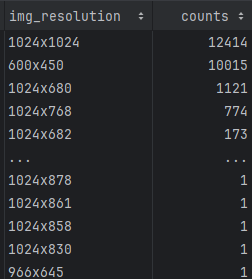
\includegraphics[scale=0.75 ]{images/Building/resolution_list.png}
        \caption{Images resolution distribution Spreadsheet.}
    \label{fig:Spreadsheet_resolution_images}
    \vspace{-100pt}
\end{wrapfigure}

In this section, the \textit{ISIC Challenge dataset}  2019 was used.  It is formed by a set of 25,331 dermoscopic images related to 8 different types of skin diseases \cite{dataset_ref_1}, \cite{dataset_ref_2} y \cite{dataset_ref_3}. The images are stored in \textbf{various resolution sizes that need to be unified into a smaller single-size}. A representation of the image resolution is given in the following table \ref{fig:Spreadsheet_resolution_images}. 

\newpage
As these are real patient images, we also encounter other shapes and features, such as hair, lesion markers, and other objects that can distort the sample.

The dataset used for this research implies a larger quantity of one specific kind of images that causes an imbalance concerning the proportion of the total images quantity in each class, being Nevus, the one with the biggest class with more than 10.000 images. Compared with DF only having 215 images, this causes an enormous disparity. Figure \ref{fig:class_distribution_for_train} shows how the different classes are distributed across the dataset. 

\begin{figure}[ht]
    \centering
        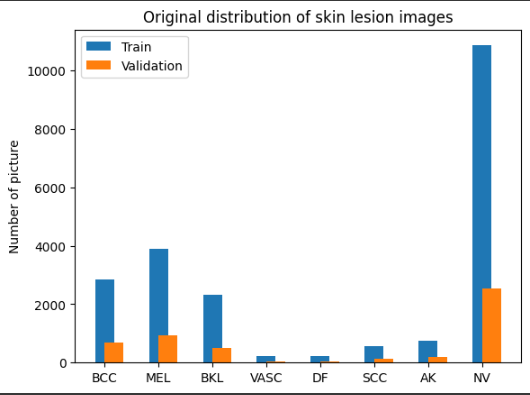
\includegraphics[scale=0.75]{images/Building/Original_distribution_skin_lesion_images.png}
        \caption{Original class distribution for training.}
    \label{fig:class_distribution_for_train}
\end{figure}


A disproportioned dataset could result in wrong output metrics because there is an induced bias during the network training. This might cause the network to give more importance to those classes with more weight in the dataset distribution. As a result, the lower weight classes could be ignored affecting the neural network performance. Due to all this, it is necessary to balance the dataset prior to training the neural network, so that every dataset class has the same weight, improving the network capability to learn. 

Different techniques to correct an unbalanced dataset exist, such as: 
\begin{enumerate}
    \item \textbf{Re-sampling Techniques}: Consists of applying oversampling or sub-sampling in order to make equal class proportions.    
    \item \textbf{Data augmentation}: Involves doing different copies of a picture, introducing variables such as picture proportion, brightness, color saturation, and others.
    \item \textbf{Feature selection}: Includes a careful selection of the main feature that describes the image to improve the minority classes' representation.
    \item \textbf{Sintetic image generation}: This technique involves the creation of artificial images that are very similar to the real thing.  

\end{enumerate}

The data preparation framework to be used in this work includes the \textbf{sub-sampling} and \textbf{over-sampling} phases, which will allow us to have a balanced dataset, and we will apply \textbf{data augmentation} to improve the data diversity in order to make our models generalize better avoiding the overfitting.

     
%% Data Preparation
\section{Data Preparation}
Neural networks process data in matrix format.  The size of the dataset downloaded from ISIC exceeds 2 GB of information in image format. This makes it difficult to handle as a whole. In addition, as we have seen above, these images have d\textbf{ifferent resolutions and an imbalance between the different classes} \ref{fig:class_distribution_for_train}. The high level of processing required to convert the original resolution images into matrix numbers is shown in \ref{fig: Data preparation steps}. This one is composed of five steps that will be explained as follows:

\begin{figure}[ht]
    \begin{center}
        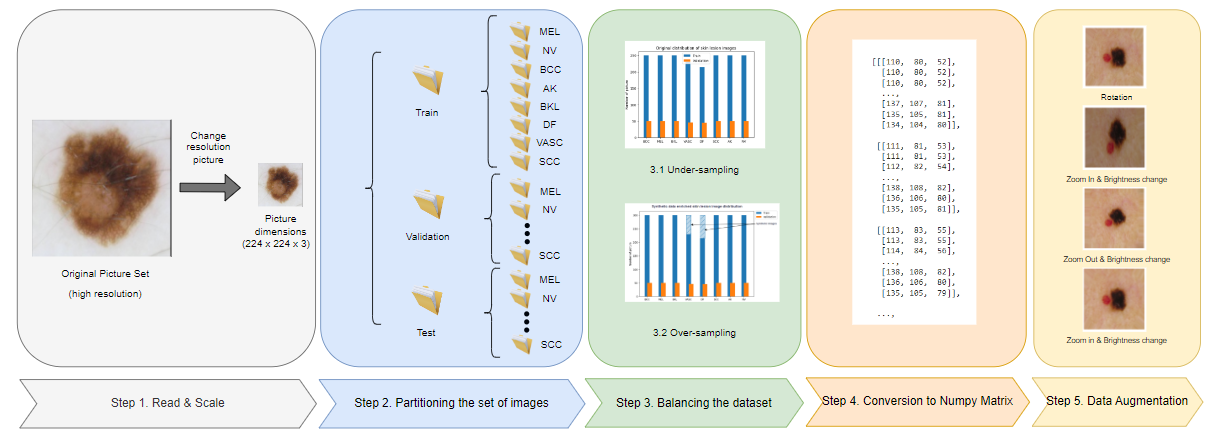
\includegraphics[scale=0.50]{images/Data_Preparation/TFM_DataPreparation_Image.png}
        \caption{Data Preparation Framework.}
    \label{fig: Data preparation steps}    
    \end{center}
\end{figure}

\subsection{{Changing image resolution (Step 1)}}
As we introduced in the previous chapter, images came originally in a wide variety of resolutions. According to that, it will be necessary to \textbf{reduce and reshape} them. So as to, make them to be the same resolution and square-shaped. The size is determined by the network used as the feature extractor. In this work, we will use EfficenteNet B0 and ResNet50 networks, which require an input size (224x244x3) corresponding to the width, height, and number of channels of the image.

\subsection{{Image set partitioning (Step 2)}}
The higher the number of images, the higher the memory consumption during the classification process. With small datasets, we would choose to load the matrices in memory, which would increase our models' training speed. With the data volume we manage in this job, however, we will have to choose \textbf{batch loading from disk}. To achieve this, the pipeline needs to classify the images according to their type by distributing them in different folders, both for training and validation.

Additionally, the batch process needs a determined folder structure to work properly. It needs the images will be classified according to their nature. During this process, the set of images \textbf{label} is determined by the name of each folder, as shown in figure \ref{fig: Data preparation steps}, step two.

The test dataset provided by ISIC 2019 does not have the labels to identify the type of lesion, and therefore, we cannot validate the performance of our models at the end of our work. Consequently, we will generate a test dataset from the original training set, randomly selecting a certain number of images for each class.


\subsection{{Balancing the dataset(Step 3)}}
As we have seen above in the description of the dataset, it is extremely important to work with a dataset in which all the classes are represented in the same proportion, in what is known as class balancing. This avoids introducing important \textbf{biases} that could lead to errors in the interpretation of the results and, especially when working with neural networks, avoids overfitting the training. As we indicated in the previous section, there are different techniques for managing a dataset with low representation in some of the classes. In this paper, we will use \textbf{under-sampling}, together with \textbf{synthetic image generation}, and a third, \textbf{data augmentation}, which we will apply at a general level to avoid network specialization. Additionally, an \textbf{over-sampling} process based on SMOTE will be used. This will be carried out in parallel in order to study the impact of introducing new synthetically generated images.

\begin{enumerate}
    \item \textbf{under-sampling}
        To obtain a balanced dataset, we apply a trim to the majority classes so they can be made equal in size.  We will apply a \textbf{random selection} to the samples of each class because we want to preserve the richness of having samples from different hospitals.

        \begin{figure}[ht]
            \begin{center}
                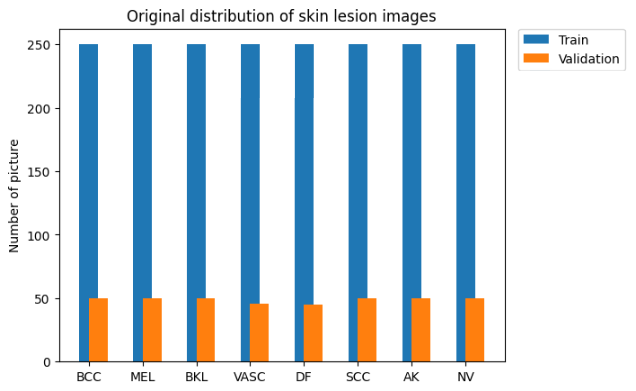
\includegraphics[scale=0.5]{images/Building/Skin lesion Balance distribution.png}
                \caption{Skin Lesions balance distribution after applying a reduction on majority classes.}
            \label{fig: Skin Lesions balance distribution}    
            \end{center}
        \end{figure}
        
    In the picture, we can see the result of applying the trimming in each of the classes. The number of images to keep per class is determined by the number of minority classes, and the limit will be set at 250 images per class.
        

    \item \textbf{Synthetic image generation} 
        \label{pr: synthetic_image_generation}
        Applying trimming to the dataset will allow us to have a balanced dataset, but on the other hand, we will lose statistical diversity in the data by discarding images of the majority classes. Using techniques such as data augmentation, also used in this work, allows us to add variation to the data and avoid specialising the network. However, an alternative solution, which also increases the statistical richness, is to \textbf{artificially increase the data set of the minority classes}. This is the purpose of the \textbf{SMOTE procedure}, which will be the subject of a more detailed discussion later in this paper.
    
\end{enumerate}

\subsection{{Image conversion to matrix (Step 4)}}
Since images are made up of pixels, their colors are constituted by numbers. For this work,  they are specifically represented in RGB encoding. This means that each pixel has a numerical translation ranging from 0 to 255 values. Depending on the feature extractor used, the values of the numerical matrix have to be \textbf{normalized} between 0 and 1 or between -1 and 1. 

\subsection{{Data Augmentation (Step 5)}}
Small data sets are often used to train neural networks. This means that the network tends to \textbf{specialize} immediately due to the small variety of data, in a process called \textbf{overfitting}. With the data augmentation technique, we generate a \textbf{series of derived images} from an original one. We have applied to them shifts, rotations, zooms, splits, or changes in brightness or color saturation to obtain new pictures. This makes the dataset richer and increases the number of images to train. As a demonstration of this, we have applied the transformations that we will perform on all the images in the training dataset to a random image in the figure \ref{fig: Data augmentation examples}.

\begin{figure}[ht]
    \begin{center}
        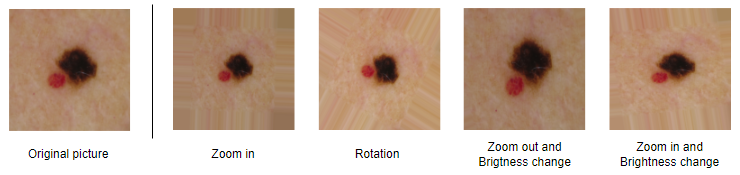
\includegraphics[scale=0.8]{images/Building/Data augmentation.png}
        \caption{Data augmentation examples.}
    \label{fig: Data augmentation examples}    
    \end{center}
\end{figure}

\subsection{Synthetic image generation} 

As we saw earlier at \ref{pr: synthetic_image_generation} when working with an unbalanced dataset, it is necessary to apply a number of pre-processing techniques to achieve a balance between the classes that make up the dataset. One of the ways to rebalance the dataset is to use oversampling by generating new samples.  To do this, we will use the Synthetic Minority Oversampling Technique, or SMOTE \cite{smote_belharar_enhancing_2023} \cite{smote_JMLR:v18:16-365} \cite{smote_maklin_synthetic_2022}, to add new images to the minority classes. 

\begin{figure}[ht]
    \begin{center}
        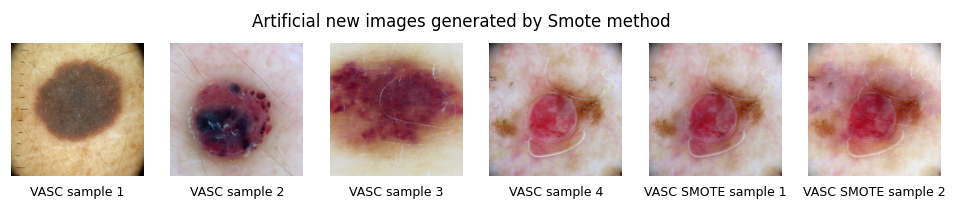
\includegraphics[scale=0.6]{images/Building/SMOTE/Smote_examples.png}
        \caption{Example of SMOTE generated synthetic images.}
    \label{fig: Smote_examples}    
    \end{center}
\end{figure}

The idea behind SMOTE is to identify the nearest neighbors of the sample and \textbf{interpolate new data} along the line connecting the sample to its neighbors according to a random value. Thus, this new synthetic data will have attributes of the original data and its neighbors while generally retaining visual features, texture, and spatial information \cite{smote_belharar_enhancing_2023}. The percentage of inherited features will depend on the proximity of the new data to the sample or neighbor. 

\begin{figure}[ht]
    \begin{center}
        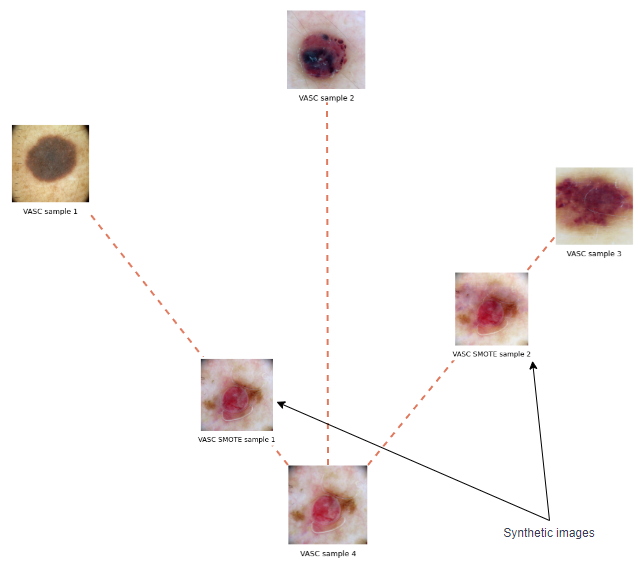
\includegraphics[scale=0.6]{images/Building/SMOTE/Smote_examples_knn.png}
        \caption{Synthetic image generation representation in 2D space}
    \label{fig: Smote_knn_representation}    
    \end{center}
\end{figure}

To better understand this concept, the above has been illustrated in figure \ref{fig: Smote_knn_representation}, where the base image has been linked to its three neighbors, as well as the artificially generated images along the imaginary line connecting them. The generated image 1 (\textit{VASC SMOTE sample 1}) has been placed very close to the base image because it shows only very slight color changes. On the other hand, the second image (\textit{VASC SMOTE sample 2}) has characteristics of both the base image and the neighbor \textit{VASC SMOTE sample 3} and is closer to the last one.



\begin{figure}[ht]
    \begin{center}
        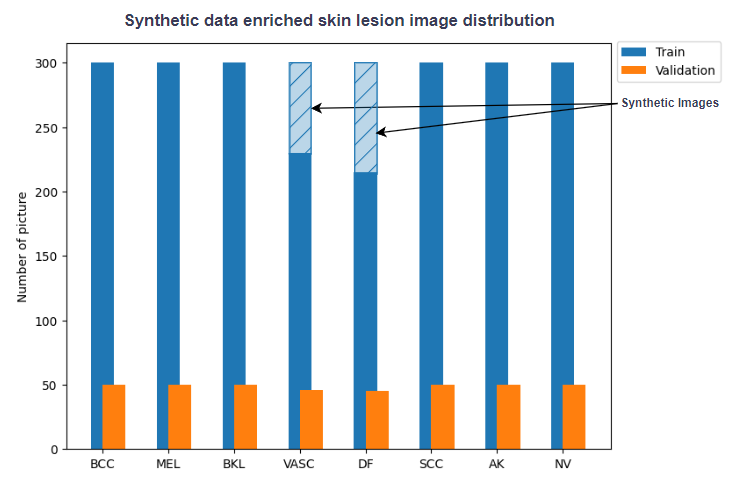
\includegraphics[scale=0.6]{images/Building/SMOTE/synthetic_data_distribution.png}
        \caption{Synthetic data distribution between minority classes}
    \label{fig: Smote_data_representation}    
    \end{center}
\end{figure}

In order to test whether it is possible to use SMOTE to improve classification efficiency, two variations of the same experiment are generated. In the first, where no synthetic samples are used, we will train the convolutional networks using a subsampling of the majority classes, setting the number of samples to 250 for each class, as shown in the figure \ref{fig: Skin Lesions balance distribution}. In a second variation, we will increase the size of each class to 300 images, and using SMOTE, we will synthetically generate 150 samples in the minority classes until the defined level is reached. A representation of the distribution of data for each class can be seen in the figure \ref{fig: Smote_data_representation}.

\begin{wrapfigure}{r}{0.50\textwidth} 
    \vspace{-40pt}
    \centering
        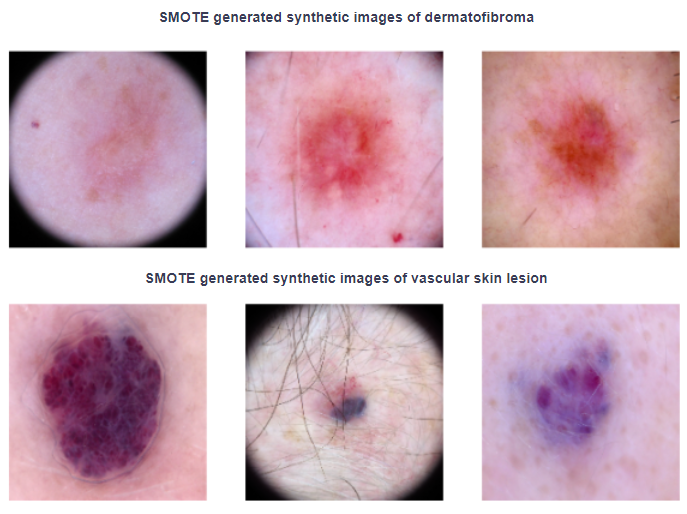
\includegraphics[scale=0.4]{images/Building/SMOTE/Artificial_new_images_generated_by_Smote.png}
        \caption{Artificial sampling generated by SMOTE }
    \label{fig: Artificial_sampling_generated_SMOTE}    
    \vspace{-100pt}
\end{wrapfigure}

\hspace{1cm}

At the end of the process described above, the synthetically generated images are stored on disk to make them available for further training. Three random samples were taken from each minority class, and the result can be observed in figure \ref{fig: Artificial_sampling_generated_SMOTE}.

\newpage
%% Looking for the best model
\section{Looking for the best model}

In this chapter, the most practical, the training of convolutional neural networks for skin lesion classification will be carried out. Two of the best-known networks will be used: EfficientNet in its less complex version (B0) and ResNet50.   

First, we will introduce the main components of this type of classification network: the feature extractor and the classification layer. The section will be illustrated with a representation of one of the networks used, the ResNet50, together with the classification block used during the training process. 

In the following, we will describe the learning process that we will use during training. With this process, we will train the network to use the knowledge learned by the feature extractor to distinguish shapes and contours by transferring the weights of Imagenet, a dataset consisting of more than 1000 labeled classes with a total of 14 million images.

In the following section, the hyperparameters of the network are searched. This is the first step that any model must go through before being trained, and it consists of studying the network's behavior during short training sessions while varying the training parameters. This will allow us to decide on the best combination of parameters to use during the training process. 

Finally, the chapter will conclude by describing the results of the training processes with the two networks used in this work, \textbf{EfficientNet B0} and \textbf{ResNet50}.

\subsection{Image classification model assembly}

As we have seen throughout this thesis, convolutional neural networks (ConNet) are widely used in image classification processes. These networks are decomposed into two stages: 

\begin{enumerate}
    \item The \textbf{feature extractor}, the first stage, is responsible for detecting patterns in the image whose complexity increases as we deepen the network. 
    \item The second stage is applied for the  \textbf{classification layer} is connected to the output of the feature extractor and is responsible for determining the class to which the input belongs.
\end{enumerate}


\begin{figure}[ht]
    \begin{center}
        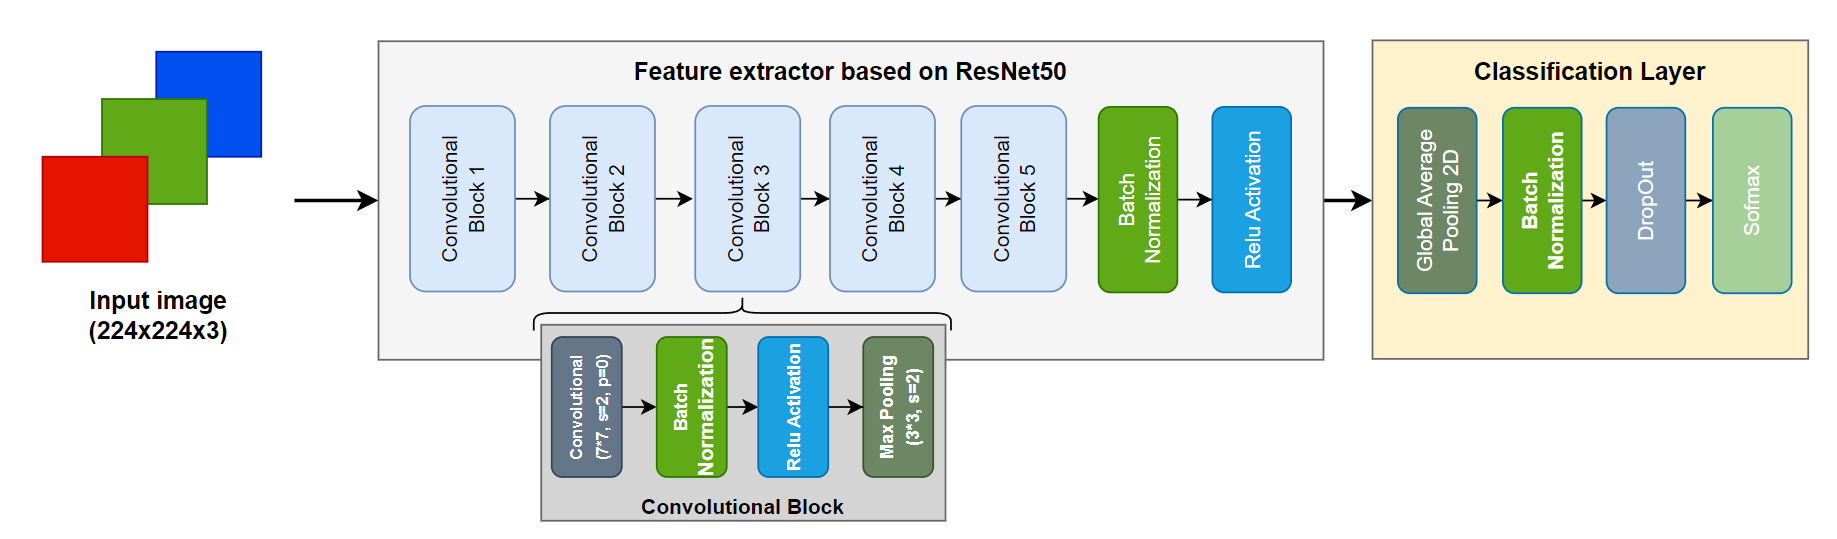
\includegraphics[scale=0.35]{images/Building/Transfer learning/Ensambled Model.png}
        \caption{ResNet50-based assembly model used for testing}
    \label{fig: Ensamble_Model_RNet50}    
    \end{center}
\end{figure}

The figure \ref{fig: Ensamble_Model_RNet50} shows the two stages discussed above. For the feature extractor stage, also called the \textbf{base model}, the RedNet50 network map used in this project was chosen. The other network, \textit{EfficientNet}, changes the number of convolutional blocks used and their composition, but the construction scheme follows the same pattern for didactic purposes. 

The \textbf{base model}, based on ResNet50, consists of five convolutional blocks, followed by a batch normalizing layer and activated by ReLu. \textbf{Batch normalization} layers calculate the mean and standard deviation of a batch during the training process, ensuring the stability of the network by centering and normalizing each mini-batch of data, which is placed in front of an activation function, as shown in the figure. In contrast, the \textbf{ReLu activation} function is used to bring the network into non-linearity. This function, which is very common in neural networks, is responsible for initializing the negative values of the layer's input function to zero. On the other hand, each block contains a convolutional layer with a 7x7 kernel, a stride set to two and no padding, a batch normalization layer, a layer applying the ReLu function, both described above and a \textbf{max-pooling layer}. This last layer is responsible for reducing the dimensionality by selecting the maximum value of the region in which it operates, which, in the case of the convolutional blocks of ResNet50, corresponds to a 3x3 matrix.

The second stage of the model, the classification module, assigns labels to the feature extractor's output results. This stage consists of four layers: The operation of the first of these, \textbf{Global Average Polling 2D}, is very similar to Max Pooling above, except that it calculates the average of all input values for each channel. This reduces the dimensionality of the number of channels in the input layer. The second layer, the Bach normalization, was explained in the previous section. Following this is a \textbf{dropout layer}, which randomly deactivates certain neurons during each iteration. This introduces randomness to the training process and reduces the risk of overfitting. In this paper, the dropout rate has been set to 0.2, meaning that 20\% of the neurons will be deactivated. Finally, the classification module's last layer utilizes the \textbf{softmax} function to convert input values, known as logits, into probabilities. This ensures that the sum of the values of each class equals unity. The softmax function is commonly used in multi-class classification problems, such as the one analyzed in this paper. Its output facilitates the interpretation of the network output.

To conclude this section, we will discuss one parameter that must be chosen to train the networks. This is the \textbf{loss function}, and it is used to quantify the difference between the model predictions and the validation data. The result of this function is used to adjust the neural network weights at each training step, aiming to minimize the error obtained by the function. The function chosen for this purpose, and one of the most common in the world of deep learning, is the \textbf{categorical cross-entropy} \cite{alberto_funciones_2021}, which is described by the following formula. 

\hspace{3cm}

\hspace{5cm} $CrossEntropy = - \frac{1}{n} \sum_{j=1}^{n} \sum_{i=1}^{c} y_i log y'_i$

\hspace{3cm}

This function requires the label values to be \textbf{encoded by one-hot}. This type of encoding assigns the value 1 to the correct class, leaving the rest of the classes at 0. The nomenclature used in the above formula is as follows: "\textit{i}" represents the class, "\textit{c}" the total number of classes, "\textit{$y_i$}" is the value of the actual class and "\textit{$y'$}" the value of the predicted class. Due to the use of one-hot encoding, the calculation will be applied only to the real class, and to the value to be obtained at the output of the softmax function, reducing to zero the remaining sums of the polynomial belonging to the rest of the other classes.  



%\newpage
%% Transfer learning
\subsection{Transfer learning}

To achieve high metrics, it is necessary to train large data sets and long neural networks with many layers. An alternative to it is to use a pre-trained network with a very large dataset. This network has already learned to extract basic features from images efficiently. 

Have you ever seen a cartoonist working? He starts by drawing basic shapes, lines, circles, and ovals, and he composes the painting as an overlay of these shapes, adding shadows and gradients to simulate volume. The idea behind transfer learning is similar to this example. It consists on using this network in the first step as a pattern recognition layer, known as \textbf{a feature extractor}. The goal of this is to extract the most informative, identifying edges, corners, and blobs and extracting, at the same time, the color histogram.  As well as in this step, a data dimensionality reduction to make it suitable for the next layer. Then, the classification layer is added according to each specific categorized problem. This way, transfer learning can be applied to tasks where the dataset is not large enough to train a complete model from scratch.

Transfer learning is performed according to the following workflow:

\begin{figure}[ht]
    \begin{center}
        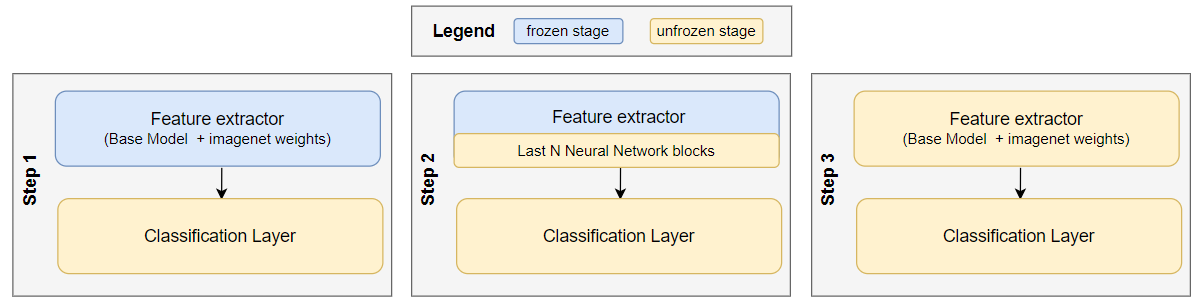
\includegraphics[scale=0.80]{images/Building/Transfer learning/Transfer Learning phases.png}
        \caption{Transfer learning phases.}
    \label{fig: Transfer learning phases}    
    \end{center}
\end{figure}

\begin{enumerate}
    \label{ch:Transfer_learning}
    
    \item In the first step, a\textbf{ pre-trained model}, which will be called the \textbf{base model}, is loaded with the training weights. This model is loaded without the classification layer (the model's top layers). The models used in this job are: \textit{Efficient B0} and \textit{ResNet 50}, both with the preloaded "\textit{ImageNet}" weights. 
 
    \item Since we want to preserve its ability as a feature extractor, we \textbf{freeze all layers} in the base model.  This way, we avoid destroying the information in future training rounds. Furthermore, a new set of trainable layers is added on top of the base model to form the \textbf{classification layer}. The whole ensemble is trained on the dataset of skin lesion images, and their weight are saved for using them in the next step. 

    \item The next step is loading an \textbf{identical model} (the feature extractor plus a classifier) with the last unfrozen feature extractor convolutional block. This new network is loaded with the weights from the previous training, and then it is trained again.

    \item Finally, we perform a fine-tuning by creating a new copy of the neural network, on which we unfreeze the whole model to retrain it with the new data using \textbf{a very low-speed learning rate}. This way, significant improvements can be achieved by adapting gradually the pre-trained features to the new data.

\end{enumerate}

\subsection{Search of Hyper-parameters}

A neural network is managed by a large number of external parameters that need to be tuned to achieve \textbf{network convergence}. This is achieved when the output of the neural network does not register significant changes even though the training process continues, maintaining the weights and biases without significant changes. Thus, Hyperparameter search is the process of finding the optimal set of parameters that define the model to obtain the best metrics but also to achieve convergence in the shortest possible time.

The parameters that will be adjusted in our work, and that are generally used in the majority of deep learning networks are described as follows:

\begin{enumerate}
    \item \textbf{Learning Rate}: It controls how much the model parameters are adjusted at each training step. A high learning rate can cause the model to converge quickly, but there is also a risk the network may be lost in a global minimum and it will not be able to complete its learning. Besides that, a low learning rate may lead to slow convergence or no convergence at all.

    \item \textbf{Epochs number}: This parameter controls the number of times the learning algorithm iterates over the entire training data set. During each epoch, the weights of the neural network are updated in an attempt to minimize the Loss function, thus improving the network learning process for each epoch. The most common values for this parameter are 16, 32, and 64, and it will always be expressed in multiples of two.

    \item \textbf{Batch Size}: The number of training samples used in a model update iteration. Its value and the dataset size determine the number of iterations required to complete an epoch. If its value is low, the model may not have enough time to learn the data patterns. On the contrary, a high epoch value may cause the model to be susceptible of overfitting by incorporating data noise into the adjustment weight.

    \item \textbf{The optimizer}: It is the element responsible for calculating the cost function gradient in each network parameter/dimension. It is an algorithm that tries to minimize the error function by searching the minimum of this function. Therefore, it is a crucial element in the network learning process, and its choice will determine the network performance. There are several \textbf{gradient descent optimizers} in the market, but in this research, we have chosen three of the most used in classification works: \textbf{SGD}, \textbf{RMSProp} and \textbf{Adam}.

    \textbf{Stochastic Gradient Descent} (SGD): This optimizer limits the gradient calculation to one per batch. It is used as a baseline in order to compare it with the others.

    \textbf{RMSProp}: Just as the SDG optimizer performs the descent gradient over a batch. This second optimizer uses the gradient-weighted average calculations over a set of samples.  This optimizer introduces variability into the training factor concept at each iteration, unlike the SGD optimizer, which keeps it stable.

    \textbf{AdaGrad}: Even if we will not use this optimizer for the current job, it is important to mention it because it adapts the learning rate for each parameter individually based on the historical gradients, making it particularly suitable for sparse data. Compared to SGD, Adagrad adjusts learning rates per parameter, sharing similarities with RMSProp. 
    
    \textbf{Adaptative moment estimation} (Adam): It inherits and combines the improvements of the AdaGrad and RMSProp algorithms while bringing in a gradient impulse averaging. This is similar to AdaGrad but performs the training factor scaling by a different formula (the exponential decay of the square of the gradients).

    Furthermore, the behavior of SDG and RMSProp optimizer can be improved using the \textit{\textbf{momentum}} parameter. This one is used to accelerate the gradient descent and soften its oscillations \cite{SGDwithMomentum}. A reference value of 0.9 is used during the hyperparameter step.

    As a complement, the following reference was added \cite{optimizers1} showing the different optimizers operation graphically, as well as their corresponding results. 

    In order to find the most optimal parameters to train our model, we followed a \textbf{grid search} model. Thus, we set the number of \textbf{epochs up to 32} since this value is the most frequently used as a starting point. From this point on, we will try different learning rate combinations and optimizers.

\end{enumerate}

\begin{figure}[ht]
    \begin{center}
        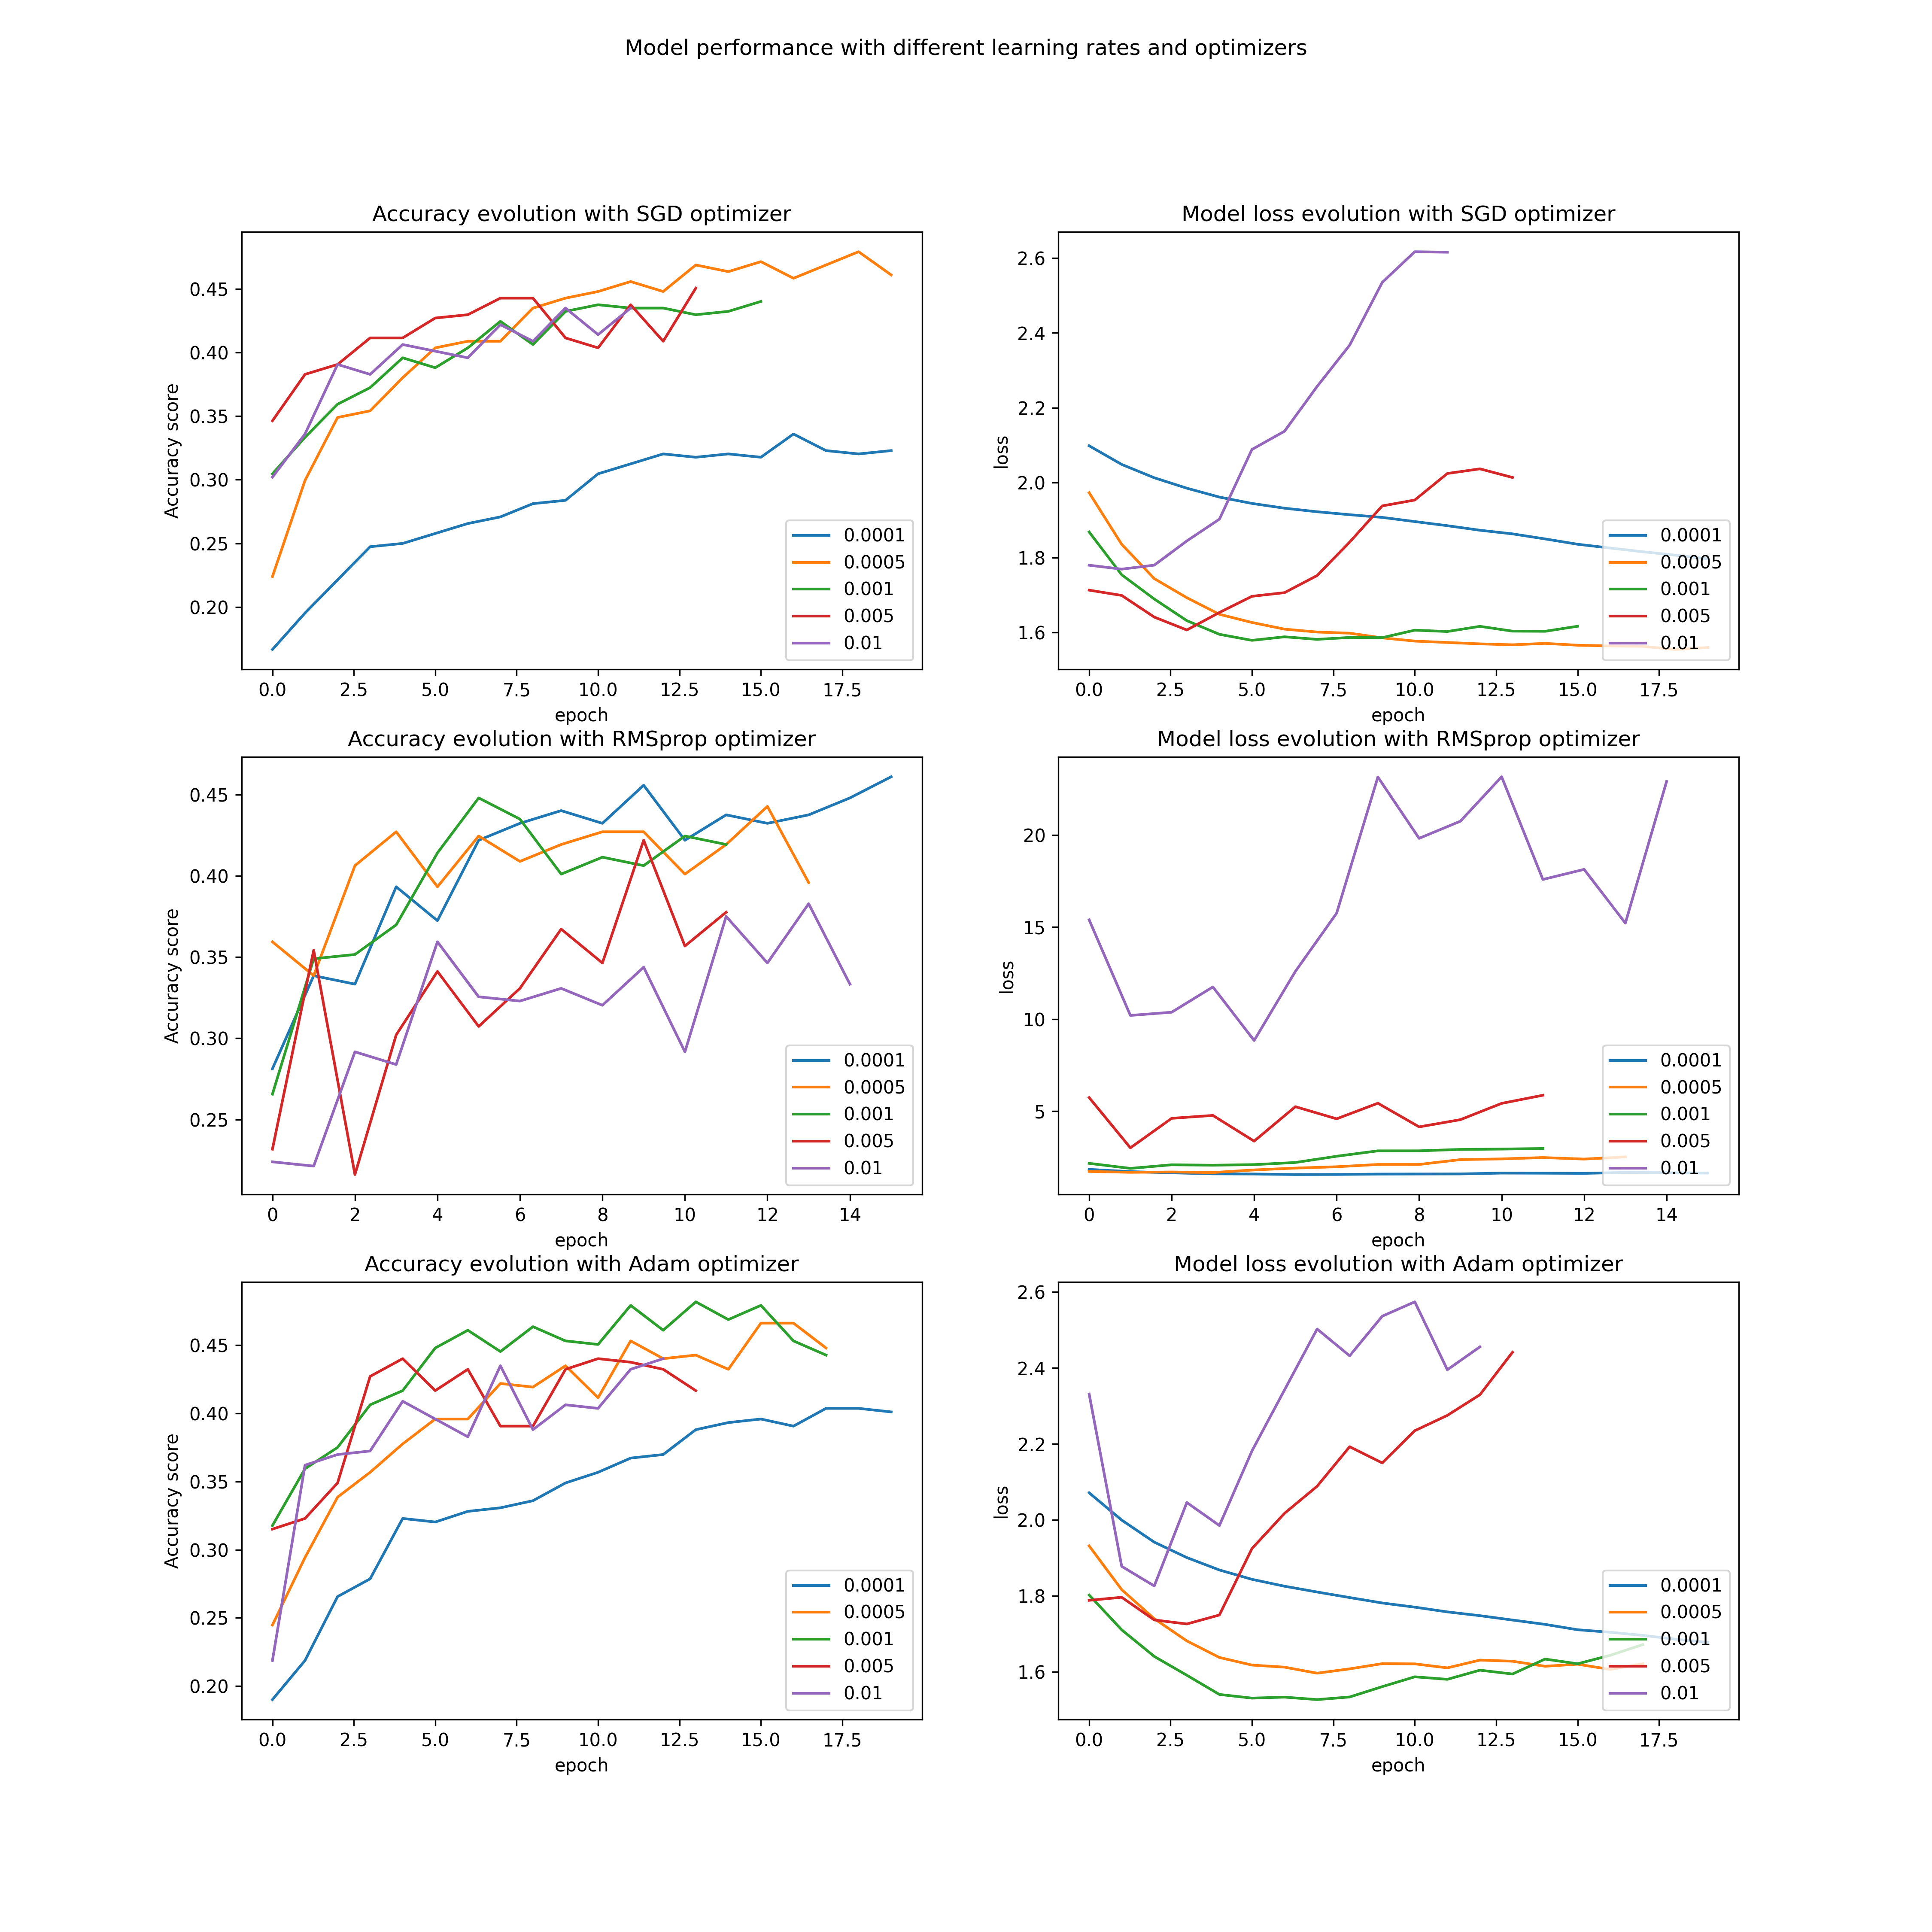
\includegraphics[scale=0.35]{images/Building/Hyperparameters/Model performance with different learning rates and optimizers.png}
        \caption{Efficient B0 base model hyperparameters search.}
    \label{fig: EfficientB0_hyperparameters}    
    \end{center}
\end{figure}

As shown in figure \ref{fig: EfficientB0_hyperparameters}, training the model with a low learning rate value and SGD or Adam optimizer is the best combination to guarantee a smooth model convergence.  In the RMSProp case, the learning process seems to be more unpredictable than the previous one, and because of this, we discarded it for our job. After comparing SGD and Adam graph's results, we observed that obtained values with the\textbf{ learning rate of 0.001}, the lowest one used, guaranteeing a stable learning long last time. Considering all the previous information and discarding between these two last optimizers, we will opt for the one that reaches the convergence point faster, that is \textbf{Adam}. 

\begin{figure}[ht]
    \begin{center}
        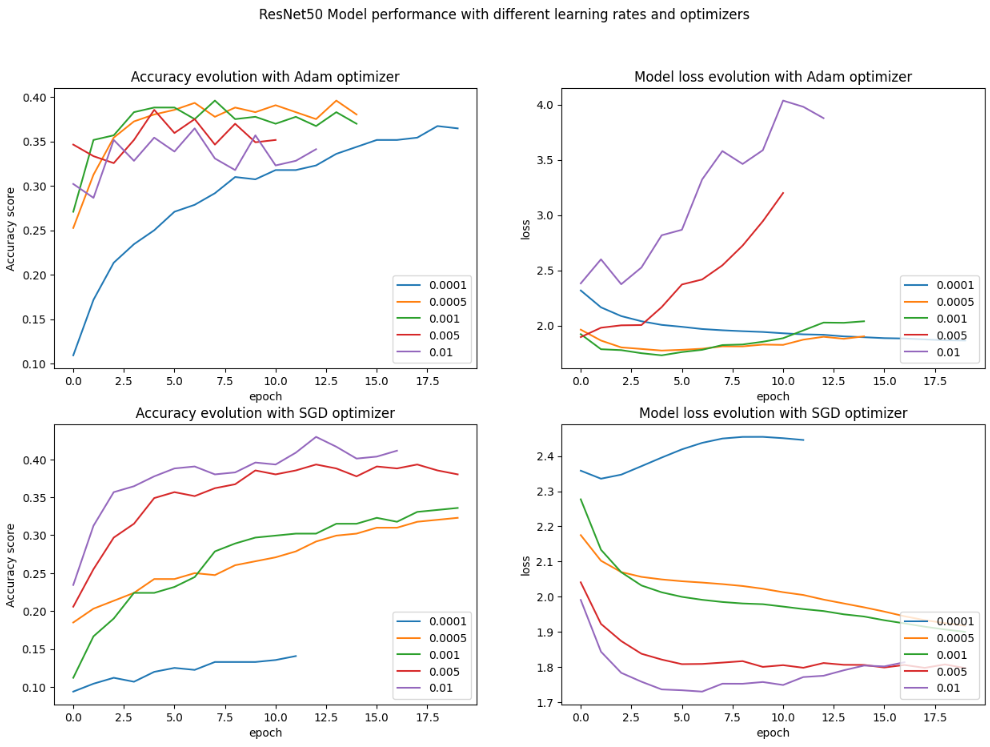
\includegraphics[scale=0.9]{images/Building/Hyperparameters/RestNet50_Model performance hyperparameters search.png}
        \caption{ResNet50 base model hyperparameters search.}
    \label{fig: ResNet50_hyperparameters}    
    \end{center}
\end{figure}

As shown in the graph \ref{fig: ResNet50_hyperparameters}, the process has also been performed in the second neuronal network based on ResNet50. In this grid search, we also used SGD, RMSProp, and Adam optimizers trained in the same learning rate range as in the previous process. As with the previous model, we discarded RMSprop from the outset because of the instability of the samples. In the case of SGD, training with the lowest learning rate values seems to offer stability, as does training with the Adam optimizer. However, we opted for the latter because we thought it would reach convergence faster. 


\newpage
\subsection{Evaluation Metrics}

Since what is not measurable cannot be improved, we define a series of metrics that will allow us to know how well our models will classify. This will help us know the progress as we move forward with the transfer learning process throughout the development of the tests. 

% Please add the following required packages to your document preamble:
% \usepackage[table,xcdraw]{xcolor}
% Beamer presentation requires \usepackage{colortbl} instead of \usepackage[table,xcdraw]{xcolor}
\begin{table}[ht]
\centering
\begin{tabular}{lclllccccc}
 & \multicolumn{9}{c}{\textbf{Prediction}} \\ \cline{3-10} 
 & \multicolumn{1}{l|}{} & \multicolumn{1}{c|}{\textbf{AK}} & \multicolumn{1}{c|}{\textbf{BCC}} & \multicolumn{1}{c|}{\textbf{BKL}} & \multicolumn{1}{c|}{\textbf{DF}} & \multicolumn{1}{c|}{\cellcolor[HTML]{C0C0C0}\textbf{MEL}} & \multicolumn{1}{c|}{\textbf{NV}} & \multicolumn{1}{c|}{\textbf{SCC}} & \multicolumn{1}{c|}{\textbf{VASC}} \\ \cline{2-10} 
\multicolumn{1}{l|}{} & \multicolumn{1}{c|}{\textbf{AK}} & \multicolumn{1}{c|}{\cellcolor[HTML]{EFEFEF}TP} & \multicolumn{1}{c|}{} & \multicolumn{1}{c|}{} & \multicolumn{1}{c|}{} & \multicolumn{1}{c|}{} & \multicolumn{1}{c|}{} & \multicolumn{1}{c|}{} & \multicolumn{1}{c|}{} \\ \cline{2-10} 
\multicolumn{1}{l|}{} & \multicolumn{1}{c|}{\textbf{BCC}} & \multicolumn{1}{c|}{} & \multicolumn{1}{c|}{\cellcolor[HTML]{EFEFEF}TP} & \multicolumn{1}{c|}{} & \multicolumn{1}{c|}{} & \multicolumn{1}{c|}{\cellcolor[HTML]{FFCE93}FP\_1} & \multicolumn{1}{c|}{} & \multicolumn{1}{c|}{} & \multicolumn{1}{c|}{} \\ \cline{2-10} 
\multicolumn{1}{c|}{\textbf{R}} & \multicolumn{1}{c|}{\textbf{BKL}} & \multicolumn{1}{c|}{} & \multicolumn{1}{c|}{} & \multicolumn{1}{c|}{\cellcolor[HTML]{EFEFEF}TP} & \multicolumn{1}{c|}{} & \multicolumn{1}{c|}{\cellcolor[HTML]{FFCE93}FP\_2} & \multicolumn{1}{c|}{} & \multicolumn{1}{c|}{} & \multicolumn{1}{c|}{} \\ \cline{2-10} 
\multicolumn{1}{c|}{\textbf{e}} & \multicolumn{1}{c|}{\textbf{DF}} & \multicolumn{1}{l|}{} & \multicolumn{1}{l|}{} & \multicolumn{1}{l|}{} & \multicolumn{1}{c|}{\cellcolor[HTML]{EFEFEF}TP} & \multicolumn{1}{l|}{} & \multicolumn{1}{l|}{} & \multicolumn{1}{l|}{} & \multicolumn{1}{l|}{} \\ \cline{2-10} 
\multicolumn{1}{c|}{\textbf{a}} & \multicolumn{1}{c|}{\cellcolor[HTML]{C0C0C0}\textbf{MEL}} & \multicolumn{1}{l|}{} & \multicolumn{1}{l|}{\cellcolor[HTML]{FFFFC7}FN\_1} & \multicolumn{1}{l|}{\cellcolor[HTML]{FFFFC7}FN\_2} & \multicolumn{1}{l|}{} & \multicolumn{1}{c|}{\cellcolor[HTML]{C0C0C0}TP} & \multicolumn{1}{l|}{} & \multicolumn{1}{l|}{} & \multicolumn{1}{l|}{} \\ \cline{2-10} 
\multicolumn{1}{c|}{\textbf{l}} & \multicolumn{1}{c|}{\textbf{NV}} & \multicolumn{1}{l|}{} & \multicolumn{1}{l|}{} & \multicolumn{1}{l|}{} & \multicolumn{1}{l|}{} & \multicolumn{1}{l|}{} & \multicolumn{1}{c|}{\cellcolor[HTML]{EFEFEF}TP} & \multicolumn{1}{l|}{} & \multicolumn{1}{l|}{} \\ \cline{2-10} 
\multicolumn{1}{c|}{\textbf{}} & \multicolumn{1}{c|}{\textbf{SCC}} & \multicolumn{1}{l|}{} & \multicolumn{1}{l|}{} & \multicolumn{1}{l|}{} & \multicolumn{1}{l|}{} & \multicolumn{1}{l|}{} & \multicolumn{1}{l|}{} & \multicolumn{1}{c|}{\cellcolor[HTML]{EFEFEF}TP} & \multicolumn{1}{l|}{} \\ \cline{2-10} 
\multicolumn{1}{l|}{} & \multicolumn{1}{c|}{\textbf{VASC}} & \multicolumn{1}{l|}{} & \multicolumn{1}{l|}{} & \multicolumn{1}{l|}{} & \multicolumn{1}{l|}{} & \multicolumn{1}{l|}{} & \multicolumn{1}{l|}{} & \multicolumn{1}{l|}{} & \multicolumn{1}{c|}{\cellcolor[HTML]{EFEFEF}TP} \\ \cline{2-10} 
\end{tabular}
    \caption{Multiclass matrix example}
    \label{tbl: Multiclass_matrix}
\end{table}

In a multiclass classification context, to visualize the successes or failures of the prediction, we compare the obtained values with the real ones in a confusion matrix, as shown in the figure \ref{tbl: Multiclass_matrix}. The main diagonal of the matrix shows the True Positives (TP). In this representation, we have focused on one of the classes (MEL) to show the False Positives (FP) or those predictions that are not correct. With the same class, we can see those images belonging to the MEL class have been classified to a different class and, therefore, will be False Negative (FN).

The main metrics to be used are the following:

\begin{enumerate}
    \item \textbf{Accuracy} (Acc):  A metric that measures a model's predictions' overall level of correctness. It is calculated as the ratio of the number of correct predictions, positive and negative, to all predictions made.    
    
    \hspace{5cm} $Acc = \frac{(TP + TN)}{(TP + TN + FP + FN)}$    
          
    \item \textbf{Precision} (Prec): Measures the proportion of correctly identified positive instances among all instances identified as positive. It is calculated as the ratio of true positives to the sum of true positives and false positives.
    
    \hspace{5cm} $Prec = \frac{(TP)}{(TP + FP)}$
          
    \item \textbf{Sensitivity} (Sen): Sensitivity measures the ability of a model to identify positive cases among all true positives. It is a metric often called Recall and is calculated as the ratio of True Positive predictions to the sum of True positive and False Negative predictions.

    \hspace{5cm} $Sen = Rec = \frac{(TP)}{(TP + FN)}$
    
    \item \textbf{Specificity} (Esp): This metric indicates the ability of a model to correctly identify negative cases out of the total number of true negatives. It is calculated as the ratio of true negative predictions to the sum of true negatives and false positives.

    \hspace{5cm} $Esp = \frac{(TN)}{(TN + FP)}$
    
    \item \textbf{F1-score} (F1): When evaluating classifiers, trying to estimate the value of false positives and negatives is sometimes complex. The F1-score metric allows us to gain insight into classifier model performance where accuracy and Recall may not represent overall model performance. This metric is calculated as the harmonic mean between precision and Recall, and thanks to this type of calculation, it is a metric that is not as affected when there are imbalances between classes. These penalizing models have unequal performance between positive and negative class identification. 

    \hspace{3cm} $F1-score = 2 * \frac{(Prec * Sen)}{(Prec + Sen)} = \frac{(TP)}{(TP + \frac{1}{2}(FP + FN)}$

    In a multiclass classification context such as the one we are working on in this article, the calculation is performed with the One-vs-Rest (OvR) strategy, in which the value is calculated for each class separately. Subsequently, the values are averaged to extract the overall value of the metric. However, we are faced with three possibilities: Performing an arithmetic average across all classes, in which case we speak of F1 calculated with Macro Average. Another option would be to use a weighted average to penalize possible imbalances in the dataset. This second case is known as the F1 Weighted Average. The third case, perhaps the most interesting of all, sums the values of TP, FP, and FN for all classes, using the second of the formulas for the calculation. This metric we will use in our study is called the F1-score for Micro Average.
    
    
\end{enumerate}
    


\subsection{Skin lesion classification with EfficientNet B0}
Traditionally, high accuracy in image classification has been achieved by increasing the number of layers in convolutional neural networks (ConNets). In 2020, Mingxing Tan and Quoc V. Le rethink the scaling-up process in this type of usage in the article "\textit{EfficientNet: Rethinking Model Scaling for Convolutional Neural Networks}" \cite{tan_efficientnet_2020}. To understand the process, we need to remember that any neural network can be characterized as three dimensions: depth, width, and resolution. In the paper cited above, the authors observe empirically that \textbf{these dimensions are not independent} and they are related to each other. Therefore, when scaling the network, \textbf{it is necessary to maintain a balance between the dimensions to achieve greater accuracy and efficiency}. For this reason, the authors propose a new composite scaling method with the aim of being able to scale the dimensions in a uniform way and thus increase the network efficiency. Finally, the work succeeds in obtaining a new neural network family model called EfficientNets, which is composed of eight variations from B0 to B7. Each variation increases the number of layers, from 213 in EfficientNet B0 to 817 in version B7 \cite{medium_EfficientNet}. 

In this chapter, we will perform transfer learning using the least parameterized network of the EfficientNet family, the B0. In order to do this, we are going to follow the steps that have been described at the beginning of the chapter \ref{ch:Transfer_learning}.


\subsubsection{Step 1. Base model froze}

As mentioned above, the 'ImageNet' weights will be loaded into the base model while the feature extractor is frozen in the first stage of the learning transfer process. Training is then performed using the optimal parameters determined during the hyperparameter search, which include a learning rate of 0.001, a batch size of 32, 40 epochs, and a patience factor of 10.

\begin{figure}[ht]
    \begin{center}
        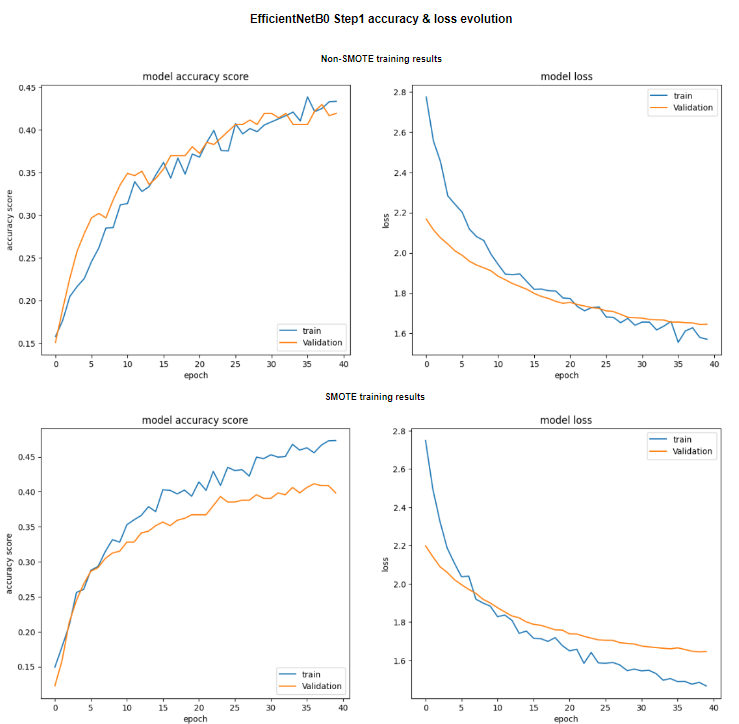
\includegraphics[scale=0.60]{images/Building/Model Efficientnet/modelENetB0_1_model accuray-loss.png}
        \caption{EfficientNetB0 model with feature extractor freeze. Accuracy-loss diagram with and without SMOTE.}
    \label{fig: Model_ENet_1_accuracy_loss}    
    \end{center}
\end{figure}

The model's training efficiently evolved and reached convergence on the 40th epoch during testing. A difference was observed when training the model using the extended dataset with synthetic images through SMOTE \ref{fig: Model_ENet_1_accuracy_loss}. In this case, \textbf{the model became more stable}, even though its training became a little slower and with a bit less accuracy for the same training time, a fact that we will better evaluate by visualizing the metric tables at the end of this section.


\begin{figure}[ht]
    \begin{center}
        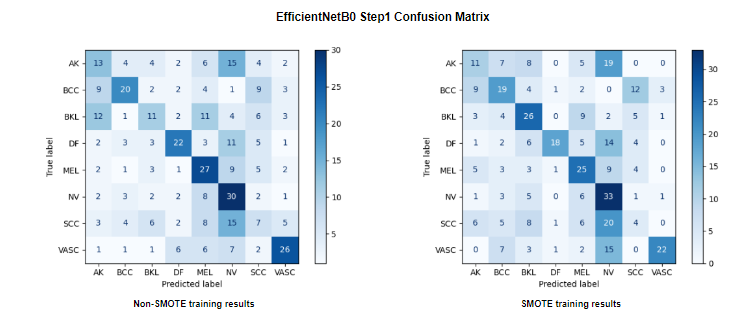
\includegraphics[scale=0.85]{images/Building/Model Efficientnet/model_ENetB0_1 Confmat.png}
        \caption{EfficientNetB0 model with feature extractor freeze. Confusion matrix.}
    \label{fig: Model_ENet_1_confmat}    
    \end{center}
\end{figure}

In figure \ref{fig: Model_ENet_1_confmat}, it is possible to compare the confusion matrices trained on the two datasets, revealing a subtle but important change when designing classifiers in the medical world, where classifiers are intended to minimize prediction errors that could lead to misdiagnosis. Thus, by examining the figure on the right, one can see \textbf{how false positives have been reduced in some of the classes}. This fact is especially relevant with VASC, where, in the SMOTE version of the dataset, these false positives decrease considerably with respect to the non-SMOTE-enriched dataset.


\begin{table}[ht]
\centering
\resizebox{\textwidth}{!}{%
\begin{tabular}{ccccccccclcccccccc}
\cline{2-9} \cline{11-18}
\multicolumn{1}{l}{} & \multicolumn{8}{c}{Values with dataset without SMOTE} &  & \multicolumn{8}{c}{Values with SMOTE dataset} \\ \cline{2-9} \cline{11-18} 
\multicolumn{1}{l}{} & \textbf{AK} & \textbf{BCC} & \textbf{BKL} & \textbf{DF} & \textbf{MEL} & \textbf{NV} & \textbf{SCC} & \textbf{VASC} &  & \textbf{AK} & \textbf{BCC} & \textbf{BKL} & \textbf{DF} & \textbf{MEL} & \textbf{NV} & \textbf{SCC} & \textbf{VASC} \\ \cline{1-9} \cline{11-18} 
\textbf{precision} & 0.30 & 0.54 & 0.34 & 0.56 & 0.37 & 0.33 & 0.18 & 0.60 &  & 0.31 & 0.38 & 041 & 0.82 & 0.42 & 0.29 & 0.13 & 0.81 \\ \cline{1-9} \cline{11-18} 
\textbf{sensitivity} & 0.26 & 0.40 & 0.22 & 0.44 & 0.54 & 0.60 & 0.14 & 0.52 &  & 0.22 & 0.38 & 0.52 & 0.36 & 0.50 & 0.66 & 0.08 & 0.26 \\ \cline{1-9} \cline{11-18} 
\textbf{F1 score} & 0.28 & 0.46 & 0.27 & 0.49 & 0.44 & 0.42 & 0.16 & 0.56 &  & 0.26 & 0.38 & 0.46 & 0.50 & 0.45 & 0.41 & 0.10 & 0.57 \\ \cline{1-9} \cline{11-18} 
\end{tabular}%
}
    \caption{EffcientNet B0 Step 1. Metrics obtained by class.}
    \label{tbl: Model_ENet_1_class_values}
\end{table}

The table \ref{tbl: Model_ENet_1_class_values} shows the numerical representation of each metric for each of the classes. As mentioned in the previous paragraph, when looking at the confusion matrices, we see a 21\% increase in classification accuracy for the VASC class when using SMOTE, as well as for the DF class, which has a significant increase in this metric. However, the F1 score for both classes increases by one percentile due to the decrease in sensitivity.  Let us remember that the F1 metric, at a general level, will give a more balanced indication of the classifier's ability to discriminate between healthy and sick people, taking into account both the correct positive predictions and the ratio of all positive predictions, whether true or not. This statement can also be seen in the table \ref{tbl: Model_ENet_1_global_values}, where despite a 5-point increase in accuracy obtained by training with the SMOTE-treated dataset, it only translates into a slight increase of one point in its F1-score.

% Please add the following required packages to your document preamble:
% \usepackage{graphicx}
\begin{table}[ht]
\centering
\begin{tabular}{lcccc}
\cline{2-5}
\multicolumn{1}{l}{} & \textbf{Accuracy} & \textbf{Precision} & \textbf{sensitivity} & \textbf{F1-score} \\ \hline
Values without SMOTE dataset & 0.39 & 0.40 & 0.39 & 0.38 \\ \hline
Values with SMOTE dataset & 0.40 & 0.45 & 0.40 & 0.39 \\ \hline
\end{tabular}%
    \caption{EffcientNet B0 Step 1. Global Metrics.}
    \label{tbl: Model_ENet_1_global_values}
\end{table}


\newpage
\subsubsection{Step 2. Unfroze Model base last block}

The next step to improve the metrics of our model will be to unfreeze the last convolutional block, the feature extractor, and transfer the learning obtained in step one by transferring its training weights. The base model's last convolutional block (Conv 7) is formed for 16 layers, and it has 4 more from the classification layers. For this, the total number of layers to be trained will be 20.

The training will be carried out with the next parameters: a learning rate of 0.001, a batch size of 32, and a patience factor of 10. During this stage of the transfer learning process, the model is prone to overfitting quickly. To avoid this, training is limited to eight epochs. 

\begin{figure}[ht]
    \begin{center}
        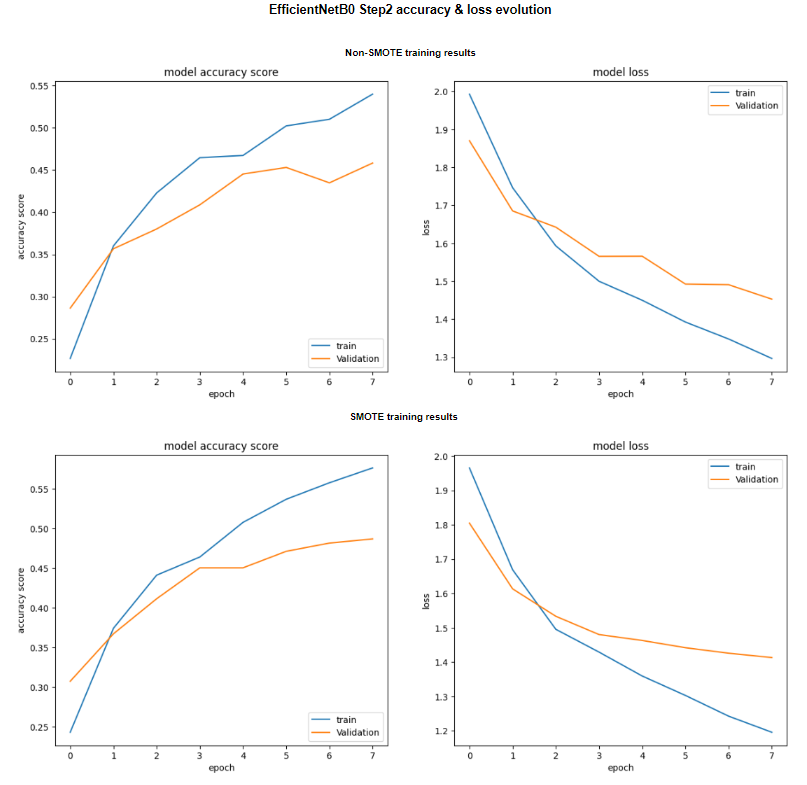
\includegraphics[scale=0.6]{images/Building/Model Efficientnet/modelENetB0_2_model accuray-loss.png}
        \caption{EfficientNetB0 model with the last block unfroze. Accuracy-loss diagram.}
    \label{fig: Model_ENet_2_accuracy_loss}    
    \end{center}
\end{figure}

Examining the graphs of the training with both datasets \ref{fig: Model_ENet_2_accuracy_loss}, we also observe that although the metrics obtained are similar, the model trained with the SMOTE dataset shows more regularity. This can be followed in epoch six, in the graph showing the accuracy, and in epoch four, in the graph showing the evolution of the loss function. 


\begin{figure}[ht]
    \begin{center}
        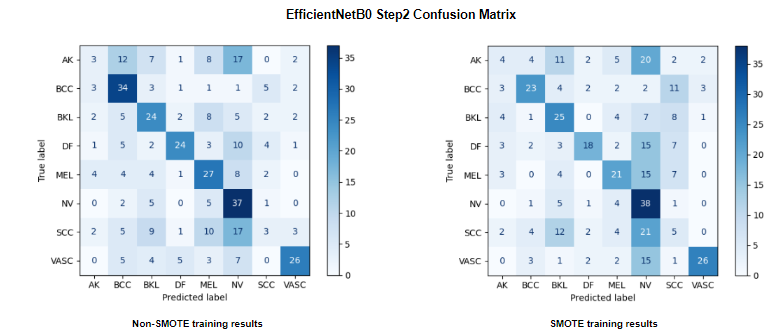
\includegraphics[scale=0.80]{images/Building/Model Efficientnet/model_ENetB0_2 Confmat.png}
        \caption{EfficientNetB0 model with the last block unfroze. Confusion matrix.}
    \label{fig: Model_ENet_2_confmat}    
    \end{center}
\end{figure}

\hspace{1cm}
\hspace{1cm}
\hspace{1cm}
\hspace{1cm}

The comparison between the training confusion metrics \ref{fig: Model_ENet_2_confmat} of both datasets shows an increase of false positives with some classes when training the dataset with SMOTE, as is the case of BKL. 

% Please add the following required packages to your document preamble:
% \usepackage{graphicx}
\begin{table}[ht]
\centering
\resizebox{\textwidth}{!}{%
\begin{tabular}{ccccccccclcccccccc}
\cline{2-9} \cline{11-18}
\multicolumn{1}{l}{} & \multicolumn{8}{c}{Values with dataset without SMOTE} &  & \multicolumn{8}{c}{Values with SMOTE dataset} \\ \cline{2-9} \cline{11-18} 
\multicolumn{1}{l}{} & \textbf{AK} & \textbf{BCC} & \textbf{BKL} & \textbf{DF} & \textbf{MEL} & \textbf{NV} & \textbf{SCC} & \textbf{VASC} &  & \textbf{AK} & \textbf{BCC} & \textbf{BKL} & \textbf{DF} & \textbf{MEL} & \textbf{NV} & \textbf{SCC} & \textbf{VASC} \\ \cline{1-9} \cline{11-18} 
\textbf{precision} & 0.2 & 0.47 & 0.41 & 0.69 & 0.42 & 0.36 & 0.18 & 0.72 &  & 0.21 & 0.61 & 0.38 & 0.67 & 0.48 & 0.29 & 0.12 & 0.81 \\ \cline{1-9} \cline{11-18} 
\textbf{sensitivity} & 0.06 & 0.68 & 0.48 & 0.48 & 0.54 & 0.74 & 0.006 & 0.52 &  & 0.08 & 0.46 & 0.50 & 0.36 & 0.42 & 0.76 & 0.10 & 0.52 \\ \cline{1-9} \cline{11-18} 
\textbf{F1 score} & 0.009 & 0.55 & 0.44 & 0.56 & 0.47 & 0.49 & 0.09 & 0.61 &  & 0.12 & 0.52 & 0.43 & 0.47 & 0.45 & 0.42 & 0.11 & 0.63 \\ \cline{1-9} \cline{11-18} 
\end{tabular}%
}
    \caption{EffcientNet B0 Step 2. Metrics obtained by class.}
    \label{tbl: Model_ENet_2_class_values}
\end{table}

Comparing the training between the two datasets \ref{tbl: Model_ENet_2_class_values}, in general, there is no significant improvement when training with the SMOTE-enriched dataset. This is also supported by examining the global metrics \ref{tbl: Model_ENet_2_global_values}, where a metrics degradation is observed when training with this dataset.

\begin{table}[ht]
\centering
\begin{tabular}{lcccc}
\cline{2-5}
 & \textbf{Accuracy} & \textbf{Precision} & \textbf{sensitivity} & \textbf{F1-score} \\ \hline
Values without SMOTE dataset & 0.45 & 0.43 & 0.44 & 0.41 \\ \hline
Values with SMOTE dataset & 0.40 & 0.45 & 0.40 & 0.39 \\ \hline
\end{tabular}
    \caption{EffcientNet B0 Step 2. Global Metrics.}
    \label{tbl: Model_ENet_2_global_values}
\end{table}



\newpage
\subsubsection{Step 3. Unfroze the model}

During the final stage of our training, we will \textbf{unfreeze the entire model}, including both the feature extractor and the classifier, and the weights from the previous training will be loaded. In order to improve the network metrics, we will perform the training with a \textbf{lower learning rate}. In this way, the training parameters used will be similar to those used in previous training sessions, except for the learning rate, which is set at 0.0001. The training duration is fixed at 40 epochs due to overfitting appearing after this time.

\begin{figure}[ht]
    \begin{center}
        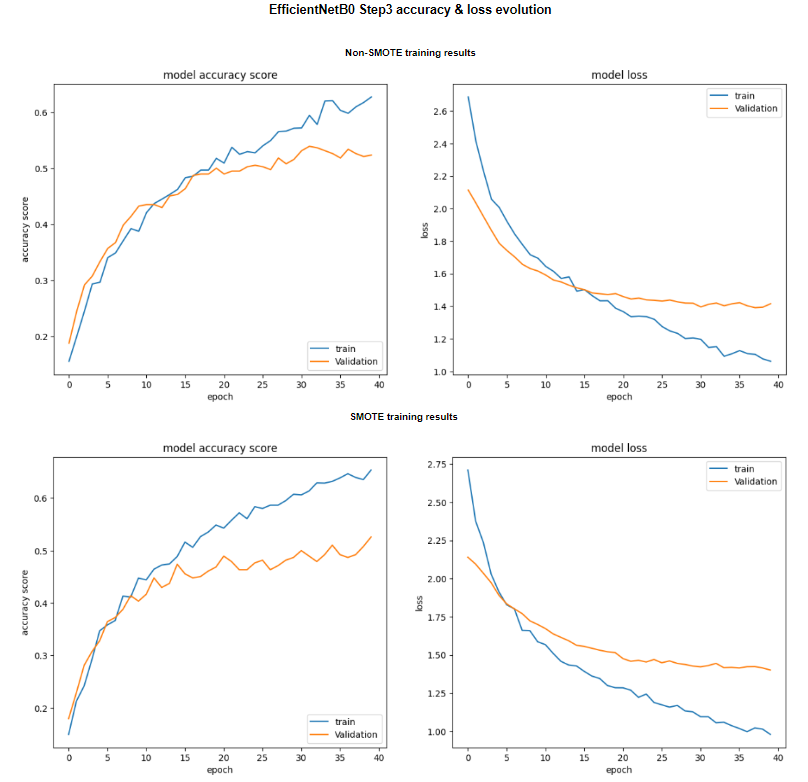
\includegraphics[scale=0.60]{images/Building/Model Efficientnet/modelENetB0_3_model accuray-loss.png}
        \caption{EfficientNetB0 model. Training all the model layers. Accuracy-loss diagram.}
    \label{fig: Model_ENet_3_accuracy_loss}    
    \end{center}
\end{figure}

The accuracy and loss function evolution graphs \ref{fig: Model_ENet_3_accuracy_loss} in this third round of training do not show a substantial difference when using one dataset or the other.


\begin{figure}[ht]
    \begin{center}
        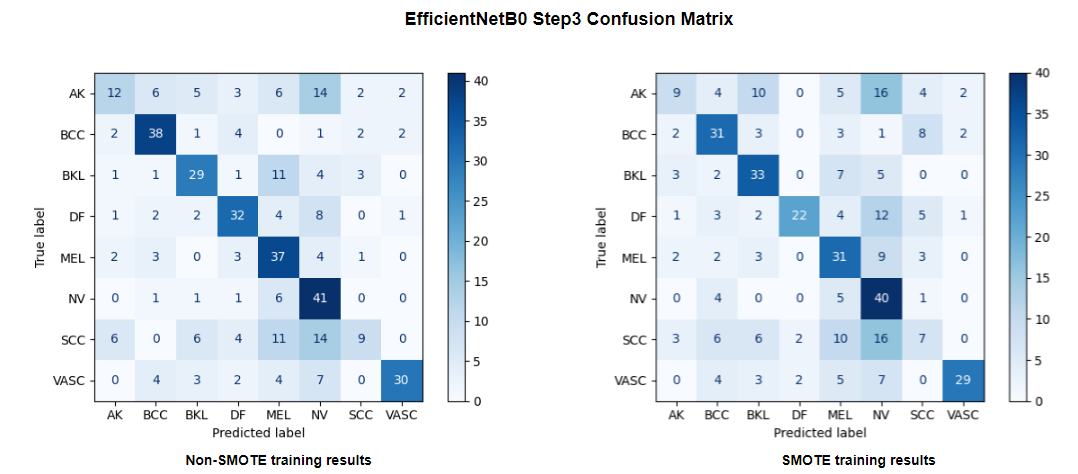
\includegraphics[scale=0.58]{images/Building/Model Efficientnet/model_ENetB0_3 Confmat.png}
        \caption{EfficientNetB0 model. Training all the model layers. Confusion matrix.}
    \label{fig: Model_ENet_3_confmat}    
    \end{center}
\end{figure}


A comparison of the confusion matrices \ref{fig: Model_ENet_3_confmat} shows that, although slightly, the \textbf{model trained with the dataset without synthetic images achieves better results}, both in identifying true positives (diagonal of the matrix) and false positives. However, if we look at the Dermatofibroma class (DF)   whose population has been synthetically increased, we can observe a considerable reduction in false positives.  

% Please add the following required packages to your document preamble:
% \usepackage{graphicx}
\begin{table}[ht]
\centering
\resizebox{\textwidth}{!}{%
\begin{tabular}{ccccccccclcccccccc}
\cline{2-9} \cline{11-18}
\multicolumn{1}{l}{} & \multicolumn{8}{c}{Values with dataset without SMOTE} &  & \multicolumn{8}{c}{Values with SMOTE dataset} \\ \cline{2-9} \cline{11-18} 
\multicolumn{1}{l}{} & \textbf{AK} & \textbf{BCC} & \textbf{BKL} & \textbf{DF} & \textbf{MEL} & \textbf{NV} & \textbf{SCC} & \textbf{VASC} &  & \textbf{AK} & \textbf{BCC} & \textbf{BKL} & \textbf{DF} & \textbf{MEL} & \textbf{NV} & \textbf{SCC} & \textbf{VASC} \\ \cline{1-9} \cline{11-18} 
\textbf{precision} & 0.50 & 0.69 & 0.62 & 0.64 & 0.47 & 0.44 & 0.53 & 0.86 &  & 0.45 & 0.55 & 0.55 & 0.86 & 0.44 & 0.38 & 0.25 & 0.85 \\ \cline{1-9} \cline{11-18} 
\textbf{sensitivity} & 0.24 & 0.76 & 0.58 & 0.64 & 0.74 & 0.82 & 0.18 & 0.60 &  & 0.18 & 0.62 & 0.66 & 0.44 & 0.62 & 0.80 & 0.14 & 0.58 \\ \cline{1-9} \cline{11-18} 
\textbf{F1 score} & 0.32 & 0.72 & 0.60 & 0.64 & 0.57 & 0.57 & 0.27 & 0.71 &  & 0.26 & 0.58 & 0.60 & 0.58 & 0.52 & 0.51 & 0.18 & 0.69 \\ \cline{1-9} \cline{11-18} 
\end{tabular}%
}
    \caption{EffcientNet B0 Step 3. Metrics obtained by class.}
    \label{tbl: Model_ENet_3_class_values}
\end{table}

An examination of the two tables \ref{tbl: Model_ENet_3_class_values} \ref{tbl: Model_ENet_3_global_values} numerically corroborates the claim that the EfficientNet B0-based model performs better with the normal dataset without synthetic sample enrichment, achieving an accuracy of 57\% with an F1-score value of 55\%.

\textbf{\begin{table}[ht]
\centering
\begin{tabular}{lcccc}
\cline{2-5}
 & \textbf{Accuracy} & \textbf{Precision} & \textbf{Sensitivity} & \textbf{F1-score} \\ \hline
Values without SMOTE dataset & 0.57 & 0.59 & 0.57 & 0.55 \\ \hline
Values with SMOTE dataset & 0.51 & 0.54 & 0.50 & 0.49 \\ \hline
\end{tabular}
    \caption{EffcientNet B0 Step 3. Global Metrics.}
    \label{tbl: Model_ENet_3_global_values}
\end{table}}

%\newpage
%\clearpage

\subsection{Skin lesion classification with ResNet50}
The second neural network we will use in this work is the one known as ResNet50, a deep neural network composed of 48 convolutional layers, more than one MaxPool, and an average pool layer, which is one of the most popular ConNets used for image classification. This network was developed in 2015 as a result of the study "\textit{Deep Residual Learning for Image Recognition}". \cite{ResNet50_2015}, in which the authors presented a residual learning framework with a deep neural network that is easily trainable and avoids the problem of gradient descent \textbf{vanishing} as the network gets deeper. Consequently, as the number of layers increases, the neural network can learn more features, but accuracy can slowly degrade due to saturation. The concept behind this neural network is the use of the residual function, which creates a shortcut to the output of the layer by adding the output of the previous layer. At depth, the residual blocks act by feeding back the gradient, preventing fading and allowing for deeper ConNets.   

\subsubsection{Step 1. Base model froze}

The strategy for training this network is the same as the one used for the EfficienteNetB0-based network. In the first step, we train with all base model layers frozen.  The training parameters to be used are a fixed learning rate of 0.001, a batch size of 32, a patience parameter of 10, and a training duration of 30 epochs. A transformation is applied to the source image matrix to ensure that the ResNet neural network has a values matrix between [-1, 1].  

\begin{figure}[ht]
    \begin{center}
        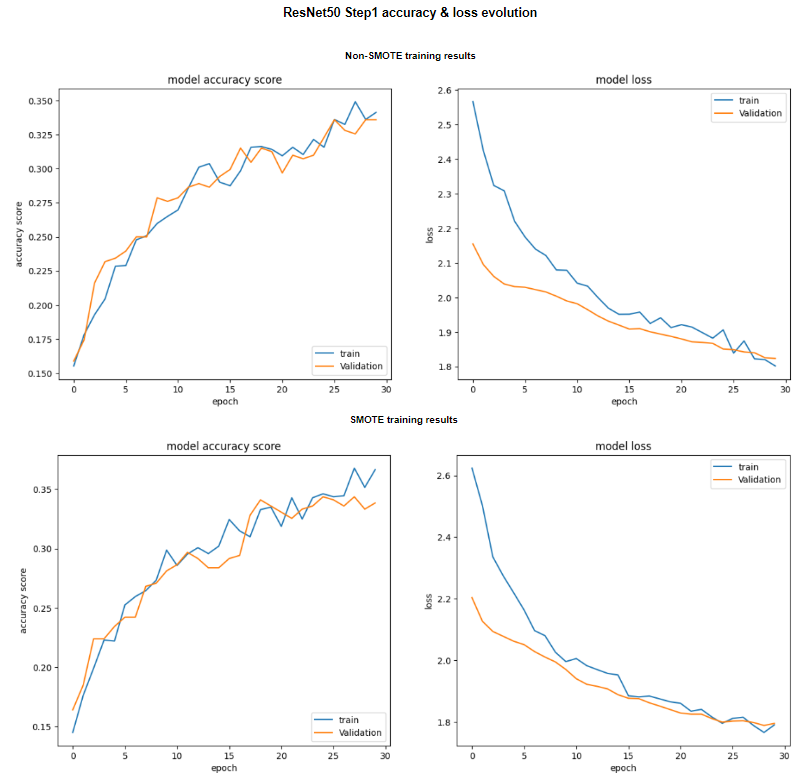
\includegraphics[scale=0.5]{images/Building/Model RestNet50/model_RNet_1_model accuray-loss.png}
        \caption{ResNet50 model with feature extractor freeze. Accuracy and loss graph.}
    \label{fig: ResNet50_1_accuracy_loss}    
    \end{center}
\end{figure}

Looking at the graph of accuracy and loss function evolution \ref{fig: ResNet50_1_accuracy_loss}, there is no significant difference between training with the SMOTE augmented dataset and the first training step with EfficientNet. Both graphs converge to the same values for similar training times, and show marked jumps in the accuracy progression. 

\begin{figure}[ht]
    \begin{center}
        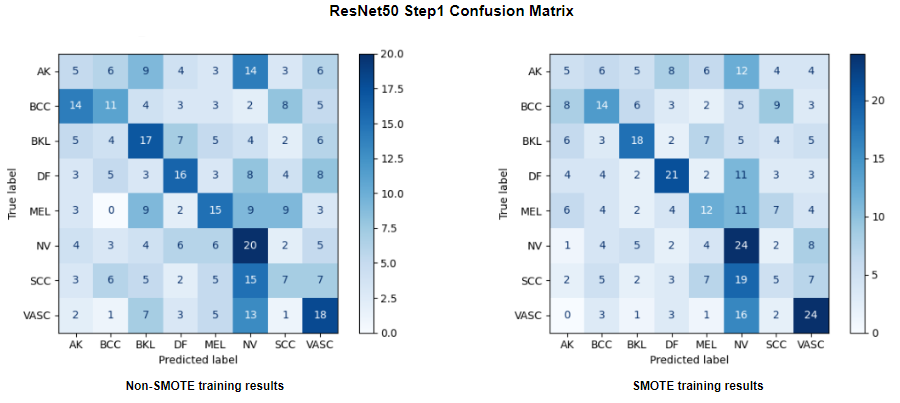
\includegraphics[scale=0.7]{images/Building/Model RestNet50/model_RNet_1 Confmat.png}
        \caption{ResNet50 model with feature extractor freeze. Confusion matrix graph.}
    \label{fig: ResNet50_1_confmat}    
    \end{center}
\end{figure}

Comparison of the confusion matrices \ref{fig: ResNet50_1_confmat} shows an improvement in accuracy, the true positives, in training with the SMOTE-enriched dataset.

% Please add the following required packages to your document preamble:
% \usepackage{graphicx}
\begin{table}[ht]
\centering
\resizebox{\textwidth}{!}{%
\begin{tabular}{ccccccccclcccccccc}
\cline{2-9} \cline{11-18}
\multicolumn{1}{l}{} & \multicolumn{8}{c}{Values with dataset without SMOTE} &  & \multicolumn{8}{c}{Values with SMOTE dataset} \\ \cline{2-9} \cline{11-18} 
\multicolumn{1}{l}{} & \textbf{AK} & \textbf{BCC} & \textbf{BKL} & \textbf{DF} & \textbf{MEL} & \textbf{NV} & \textbf{SCC} & \textbf{VASC} &  & \textbf{AK} & \textbf{BCC} & \textbf{BKL} & \textbf{DF} & \textbf{MEL} & \textbf{NV} & \textbf{SCC} & \textbf{VASC} \\ \cline{1-9} \cline{11-18} 
\textbf{precision} & 0.13 & 0.31 & 0.29 & 0.37 & 0.33 & 0.24 & 0.19 & 0.31 &  & 0.16 & 0.33 & 0.44 & 0.46 & 0.29 & 0.23 & 0.14 & 0.41 \\ \cline{1-9} \cline{11-18} 
\textbf{sensitivity} & 0.10 & 0.22 & 0.34 & 0.32 & 0.30 & 0.40 & 0.14 & 0.36 &  & 0.10 & 0.28 & 0.36 & 0.42 & 0.24 & 0.48 & 0.10 & 0.48 \\ \cline{1-9} \cline{11-18} 
\textbf{F1 score} & 0.11 & 0.26 & 0.31 & 0.34 & 0.2 & 0.30 & 0.16 & 0.33 &  & 0.12 & 0.30 & 0.40 & 0.44 & 0.26 & 0.31 & 0.12 & 0.44 \\ \cline{1-9} \cline{11-18} 
\end{tabular}%
}
    \caption{ResNet50 Step 1. Metrics obtained by class.}
    \label{tbl: Model_ResNet_1_class_values}
\end{table}

Examining the results in the table \ref{tbl: Model_ResNet_1_class_values}, it is possible to observe that all metrics results are higher for almost all classes. This fact is also observed in the table \ref{tbl: Model_RNet50_1_global_values} showing the global prediction results.

\begin{table}[ht]
\centering
\begin{tabular}{lcccc}
\cline{2-5}
 & \textbf{Accuracy} & \textbf{Precision} & \textbf{Sensitivity} & \textbf{F1-score} \\ \hline
Values without SMOTE dataset & 0.27 & 0.27 & 0.27 & 0.27 \\ \hline
Values with SMOTE dataset & 0.31 & 0.30 & 0.31 & 0.31 \\ \hline
\end{tabular}
    \caption{ResNet50 Step 1. Global Metrics.}
    \label{tbl: Model_RNet50_1_global_values}
\end{table}

Unlike the previous table, this one \ref{tbl: Model_RNet50_1_global_values} shows the indicators calculated at the global level without distinguishing between classes. It can be seen that working with the SMOTE-enriched dataset gives us a slight improvement in all the indicators. 

%\newpage
\clearpage

\subsubsection{Step 2. Unfroze Model base last block}

For the second step of the ResNet training, the feature extractor convolutional block's last layers will be unfrozen. In total, adding the last 36 layers of the convolutional block five and the 4 layers of the classifier, 40 layers of the neural model will be trained. The parameters to be used will be the same as in the previous step, except for the duration, which will be set at 5 epochs.

\begin{figure}[ht]
    \begin{center}
        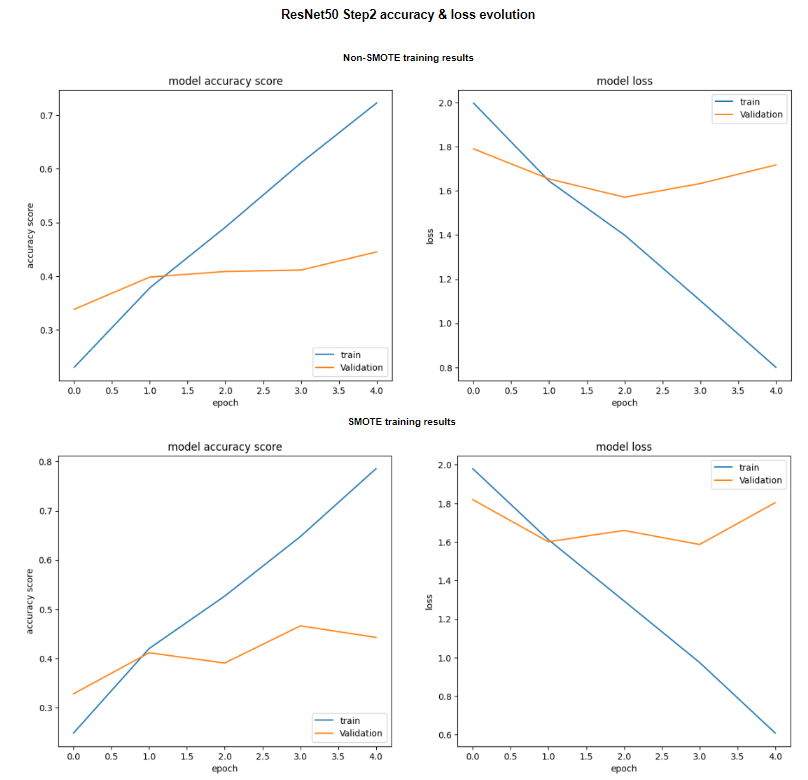
\includegraphics[scale=0.75]{images/Building/Model RestNet50/model_RNet_2_model accuray-loss.png}
        \caption{ResNet50 model with the last block unfroze. Accuracy and loss graph.}
    \label{fig: ResNet50_2_accuracy_loss}    
    \end{center}
\end{figure}

The graphs \ref{fig: ResNet50_2_accuracy_loss} show how overfitting appears already after the first training rounds, around the third epoch, with both datasets.

\begin{figure}[ht]
    \begin{center}
        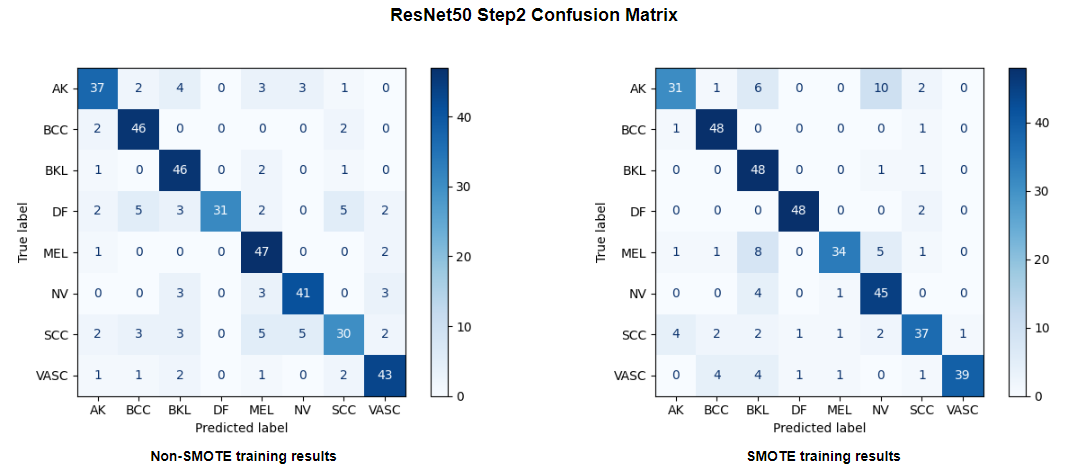
\includegraphics[scale=0.60]{images/Building/Model RestNet50/model_RNet_2_confmat.png}
        \caption{ResNet50 model with the last block unfroze. Confusion matrix graph.}
    \label{fig: ResNet50_2_confmat}    
    \end{center}
\end{figure}


The confusion matrices \ref{fig: ResNet50_2_confmat} show a very positive evolution with respect to the values obtained in step 1. The comparison between the two graphs shows that the true positives have increased significantly. For example, both \textit{Basall Cell Carcinoma} (BCC) and \textit{Benign Keratosis} (BKL) classes with the SMOTE dataset obtained 48 correct images while the values for these classes in step 1 were 14 and 18 images, respectively. False positives have also been reduced considerably, being 1 in the case of \textit{Vascular lesion} (VASC) for the dataset augmented with synthetic images.

% Please add the following required packages to your document preamble:
% \usepackage{graphicx}
\begin{table}[ht]
\centering
\resizebox{\textwidth}{!}{%
\begin{tabular}{ccccccccclcccccccc}
\cline{2-9} \cline{11-18}
\multicolumn{1}{l}{} & \multicolumn{8}{c}{Values with dataset without SMOTE} &  & \multicolumn{8}{c}{Values with SMOTE dataset} \\ \cline{2-9} \cline{11-18} 
\multicolumn{1}{l}{} & \textbf{AK} & \textbf{BCC} & \textbf{BKL} & \textbf{DF} & \textbf{MEL} & \textbf{NV} & \textbf{SCC} & \textbf{VASC} &  & \textbf{AK} & \textbf{BCC} & \textbf{BKL} & \textbf{DF} & \textbf{MEL} & \textbf{NV} & \textbf{SCC} & \textbf{VASC} \\ \cline{1-9} \cline{11-18} 
\textbf{precision} & 0.80 & 0.81 & 0.75 & 1.00 & 0.75 & 0.84 & 0.73 & 0.83 &  & 0.84 & 0.86 & 0.67 & 0.96 & 0.92 & 0.71 & 0.82 & 0.98 \\ \cline{1-9} \cline{11-18} 
\textbf{sensitivity} & 0.74 & 0.92 & 0.92 & 0.62 & 0.94 & 0.82 & 0.60 & 0.86 &  & 0.62 & 0.96 & 0.96 & 0.96 & 0.68 & 0.90 & 0.74 & 0.78 \\ \cline{1-9} \cline{11-18} 
\textbf{F1 score} & 0.77 & 0.86 & 0.83 & 0.77 & 0.83 & 0.83 & 0.66 & 0.84 &  & 0.71 & 0.91 & 0.79 & 0.96 & 0.78 & 0.80 & 0.78 & 0.87 \\ \cline{1-9} \cline{11-18} 
\end{tabular}%
}
    \caption{ResNet50 Step 2. Metrics obtained by class.}
    \label{tbl: Model_ResNet_2_class_values}
\end{table}

Examining the results by class \ref{tbl: Model_ResNet_2_class_values}, it can be seen that for some classes, better results are obtained with the dataset without SMOTE, while others obtain better results using this dataset. It is remarkable that the \textit{dermatofibroma} (DF) class, which in the first case obtained an accuracy of 100\%, but when trained with SMOTE, its sensitivity and, therefore, its F1 score increased. The opposite is the case with the \textit{vascular} (VASC) class, in which the accuracy is increased to 98\% using SMOTE, with a reduction in sensitivity. However, for this class, the classifier performs better with SMOTE, achieving an F1-score value three points higher.

\begin{table}[ht]
\centering
\begin{tabular}{lcccc}
\cline{2-5}
 & \textbf{Accuracy} & \textbf{Precision} & \textbf{sensitivity} & \textbf{F1-score} \\ \hline
Values without SMOTE dataset & 0.80 & 0.81 & 0.80 & 0.80 \\ \hline
Values with SMOTE dataset & 0.83 & 0.84 & 0.82 & 0.82 \\ \hline
\end{tabular}
    \caption{ResNet50 Step 2. Global Metrics.}
    \label{tbl: Model_RNet50_2_global_values}
\end{table}

In general, the model achieves better results when trained with the SMOTE-enriched dataset, which can be seen in the table \ref{tbl: Model_RNet50_2_global_values}. 

%\newpage
%\clearpage

\subsubsection{Step 3. Unfroze the model}
In the last step of our training, as shown in the description of the Transfer of Learning steps \ref{ch:Transfer_learning}, we will train our model in all its layers, starting from the weights inherited from the previous step and, as in step 3 of the EfficentNet training, we will do it with a lower learning rate, set to 0.0001, keeping the rest of the parameters except for the number of epochs, which will be set to eight.

\begin{figure}[ht]
    \begin{center}
        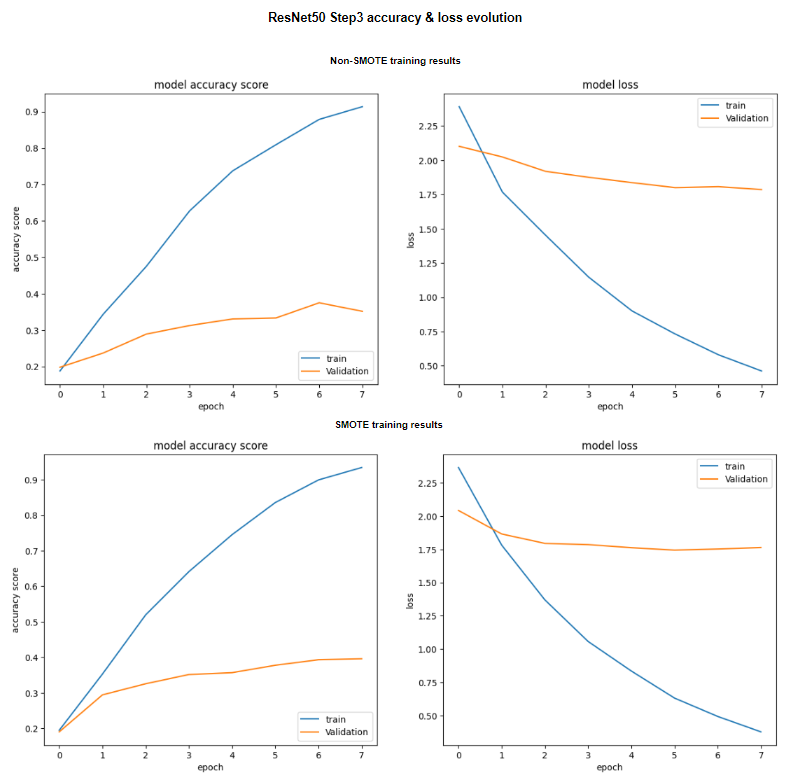
\includegraphics[scale=0.5]{images/Building/Model RestNet50/model_RNet_3_model accuray-loss.png}
        \caption{ResNet50 model. Training all the model layers. Accuracy and loss graph.}
    \label{fig: ResNet50_3_accuracy_loss}    
    \end{center}
\end{figure}

Analysis of the plots \ref{fig: ResNet50_3_accuracy_loss} shows that although the training values appear to be good if we inspect the validation data, we see that there is practically no training beyond the fifth epoch, and even though it is not shown in the tests, it was seen that the network shows overfitting from the eighth epoch and beyond.

\begin{figure}[ht]
    \begin{center}
        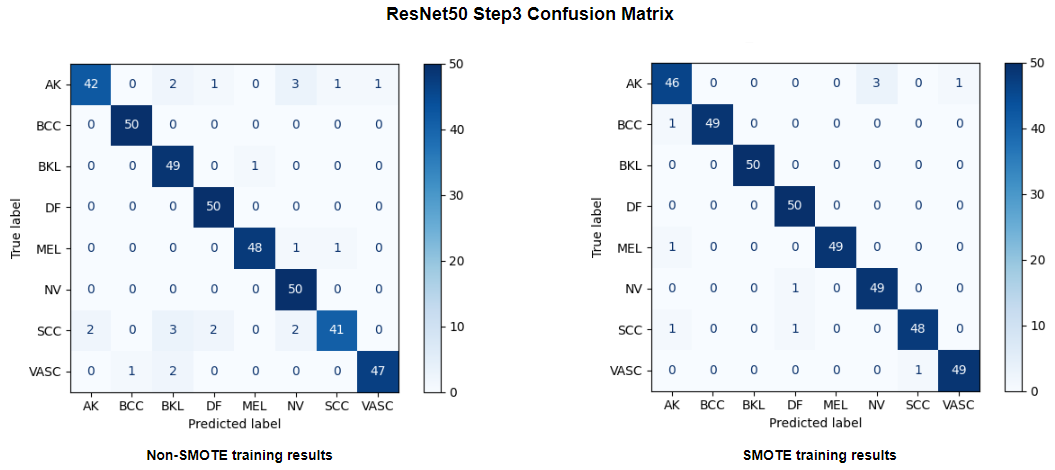
\includegraphics[scale=0.60]{images/Building/Model RestNet50/model_RNet_3_confmat.png}
        \caption{ResNet50 model. Training all the model layers. Confusion matrix graph.}
    \label{fig: ResNet50_3_confmat}    
    \end{center}
\end{figure}

The values shown by both confusion matrices \ref{fig: ResNet50_3_confmat} are similar and also very good. It is remarkable that those obtained by training with the SMOTE-enriched dataset show several classes where false positives, \textit{Basal cell carcinoma} (BBC), \textit{benign keratosis} (BKL), and \textit{Melanoma} (MEL), have been reduced to zero, and two other classes, \textit{Squamous cell carcinoma} (SCC) and \textit{Vascular lesion} (VASC), show a single case.

% Please add the following required packages to your document preamble:
% \usepackage{graphicx}
\begin{table}[ht]
\centering
\resizebox{\textwidth}{!}{%
\begin{tabular}{ccccccccclcccccccc}
\cline{2-9} \cline{11-18}
\multicolumn{1}{l}{} & \multicolumn{8}{c}{Values with dataset without SMOTE} &  & \multicolumn{8}{c}{Values with SMOTE dataset} \\ \cline{2-9} \cline{11-18} 
\multicolumn{1}{l}{} & \textbf{AK} & \textbf{BCC} & \textbf{BKL} & \textbf{DF} & \textbf{MEL} & \textbf{NV} & \textbf{SCC} & \textbf{VASC} &  & \textbf{AK} & \textbf{BCC} & \textbf{BKL} & \textbf{DF} & \textbf{MEL} & \textbf{NV} & \textbf{SCC} & \textbf{VASC} \\ \cline{1-9} \cline{11-18} 
\textbf{precision} & 0.95 & 0.98 & 0.88 & 0.94 & 0.98 & 0.89 & 0.95 & 0.98 &  & 0.94 & 1.00 & 1.00 & 0.96 & 1.00 & 0.94 & 0.98 & 0.98 \\ \cline{1-9} \cline{11-18} 
\textbf{sensitivity} & 0.84 & 1.00 & 0.98 & 1.00 & 0.96 & 1.00 & 0.82 & 0.94 &  & 0.92 & 0.98 & 1.00 & 1.00 & 0.98 & 0.98 & 0.96 & 0.98 \\ \cline{1-9} \cline{11-18} 
\textbf{F1 score} & 0.89 & 0.99 & 0.94 & 0.97 & 0.97 & 0.94 & 0.88 & 0.96 &  & 0.93 & 0.99 & 1.00 & 0.98 & 0.99 & 0.96 & 0.97 & 0.98 \\ \cline{1-9} \cline{11-18} 
\end{tabular}%
}
    \caption{ResNet50 Step 3. Metrics obtained by class.}
    \label{tbl: Model_ResNet_3_class_values}
\end{table}

The results obtained when examining the metrics for each class \ref{tbl: Model_ResNet_3_class_values} show that the F1-score reaches 100 \% in the case of \textit{benign keratosis} (BKL), and in others, it is between 98 and 99 \%. The accuracy for \textit{melanoma} detection (MEL), as well as for \textit{Basal Cell Carcinoma} (BCC) and the \textit{benign keratosis} (BKL), is 100 \%. 

\begin{table}[ht]
\centering
\begin{tabular}{lcccc}
\cline{2-5}
 & \textbf{Accuracy} & \textbf{Precision} & \textbf{sensitivity} & \textbf{F1-score} \\ \hline
Values without SMOTE dataset & 0.94 & 0.94 & 0.94 & 0.94 \\ \hline
Values with SMOTE dataset & 0.98 & 0.98 & 0.98 & 0.98 \\ \hline
\end{tabular}
    \caption{ResNet50 Step 3. Global Metrics.}
    \label{tbl: Model_RNet50_3_global_values}
\end{table}

The global metrics \ref{tbl: Model_RNet50_3_global_values} show that the classifier trained following the transfer learning process shows a better response when trained with the SMOTE-based dataset, achieving an F1-score of 98 \%.